\textbf{Herstellbare Komponenten}
\begin{itemize}[noitemsep,topsep=0pt]
    \item aktiv: Dioden, Transistoren
    \item passiv: Kapazitäten, Widerstand, Spulen (nur planar)
\end{itemize}
\end{minipage}%
\begin{minipage}{0.5\linewidth}
\begin{center}
    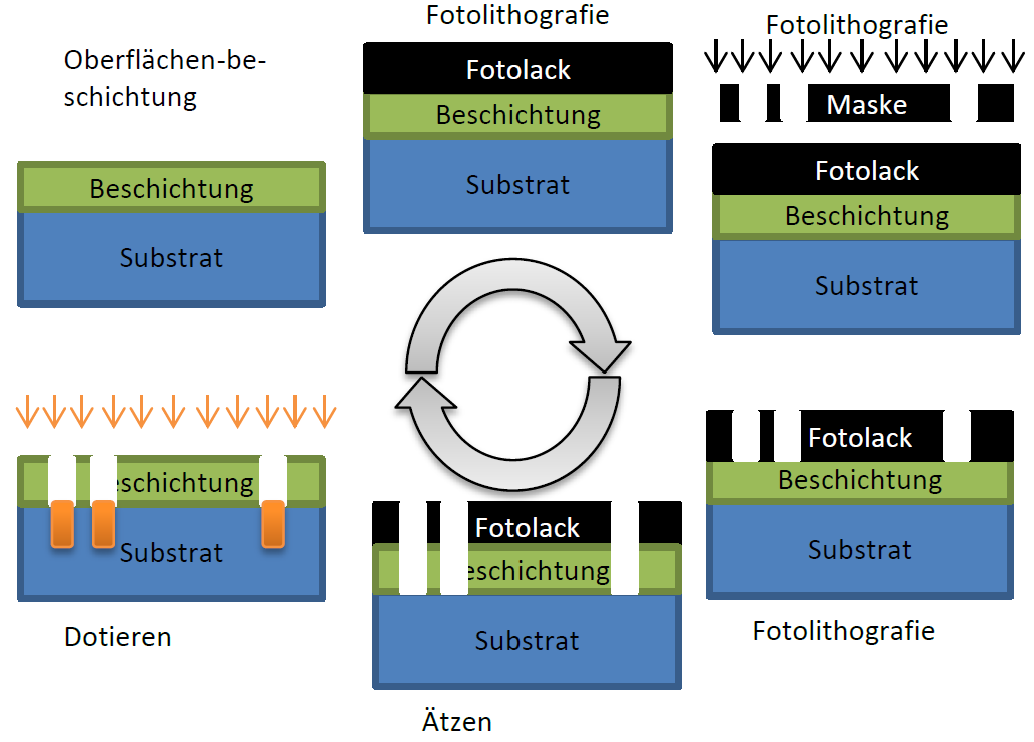
\includegraphics[width=0.8\linewidth]{Herrstellungsprozess.png}\\
\end{center}
\end{minipage}
\section{Passive Bauelemente}
\begin{minipage}{0.5\linewidth}
\subsection{Kapazität}
\boxed{C = \varepsilon\frac{A}{d} = \varepsilon\cdot\frac{W\cdot L}{d}= C'' \cdot A}\vspace{5pt}\\
\boxed{C'' = \frac{\varepsilon}{d} = \frac{\varepsilon_0\cdot\varepsilon_r}{d}}\vspace{5pt}\\ 
$[C]$ = Kapazität = $F$ \\
$[C'']$ = Kapazität/Fläche = $F/m^2$ \\
$[\varepsilon_0]$ = Permeabilität = $8.854\cdot 10^{-12}F/m$ \\
$[d]$ = Plattenabstand = $m$ \\
Poly-Poly Kap.: $C'' \approx 1fF/\mu m^2$\\
MOS Kap.: $C'' \approx 15fF/\mu m^2$  \\
MIM Kap. (MetalIsolatorMetal): $C'' \approx 1fF/\mu m^2$  \\
Siliziumdioxid: $\varepsilon_r$ = 3.9\\
Die Länge und Breite sind veränderbar. Auch die Materialkonstante ist veränderbar, dies führt jedoch zu höheren Kosten. Je tiefer die Materialkonstante ist, desto weniger Parasitäre eigenschaften tretten auf.
\end{minipage}%
\begin{minipage}{0.5\linewidth}
\subsection{Widerstände}
\boxed{R = \rho\cdot \frac{L}{A} = R_{\square} \cdot\frac{L}{W}}\vspace{5pt}\\
Nur die Länge und Breite sind veränderbar.\\
Absolute Genauigkeit:$ \pm 20 \%$,\hspace{5pt} Relative Genauigkeit:$\pm 1 \%$
\begin{center}
\begin{tabular}{|c|c|}
    \hline
    Metall                   & $R \approx 0.02...0.08\Omega/\square$ \\
    \hline
    Poly(Gate/Interconnect) &  $R \approx 10\Omega/\square$\\
    \hline
    Poly                    &  $R \approx 100...400\Omega/\square$\\
    \hline
    N-Diffusion             &  $R \approx 100\Omega/\square$ \\
    \hline
    P-Diffusion             &  $R \approx 150\Omega/\square$ \\
    \hline
    N-Well                  &  $R \approx 400\Omega/\square$ \\
    \hline
    P-Well                  &  $R \approx 1600\Omega/\square$\\
    \hline
    \end{tabular}
\end{center}
\end{minipage}\vspace{5pt}\\
\begin{minipage}{0.5\linewidth}
\section{MOS-Transistoren}
\subsection{Kennlinien}
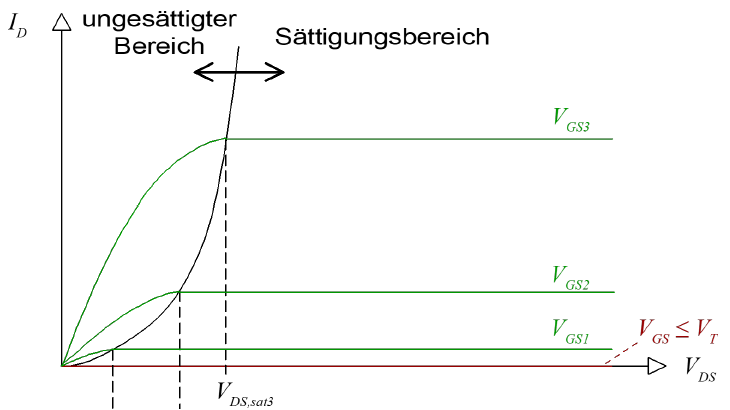
\includegraphics[width=0.6\linewidth]{Ausgangskennlinie.png}
\end{minipage}%
\begin{minipage}{0.5\linewidth}
\textbf{Gesättigt}, Stromquellen-Betrieb:\\
Gerade horizontal, dann ist $r_{\rm DS} = \infty$(idealer Transistor). Anstieg der Gerade entspricht Ausgangsleitwert $g_o$ bzw. Ausgangswiderstand $r_{\rm DS}$.\\
\textbf{Ungesättigt}, Widerstandsbetrieb:\\
Je steiler die Gerade, desto kleiner $r_{\rm DS}$.
\end{minipage}
\begin{minipage}{0.33\linewidth}
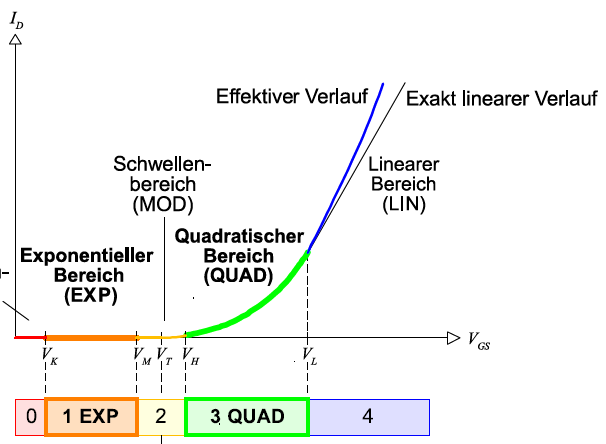
\includegraphics[width=1\linewidth]{Transferkennline.png}
\end{minipage}%
\begin{minipage}{0.33\linewidth}
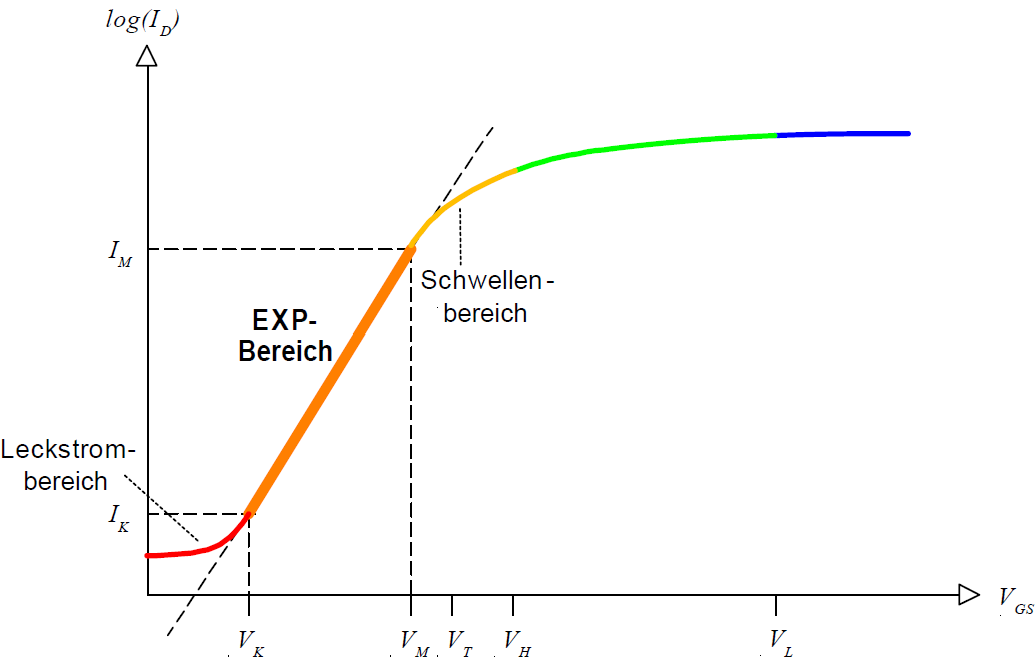
\includegraphics[width=1\linewidth]{Transferkennline_Log.png}
\end{minipage}%
\begin{minipage}{0.33\linewidth}
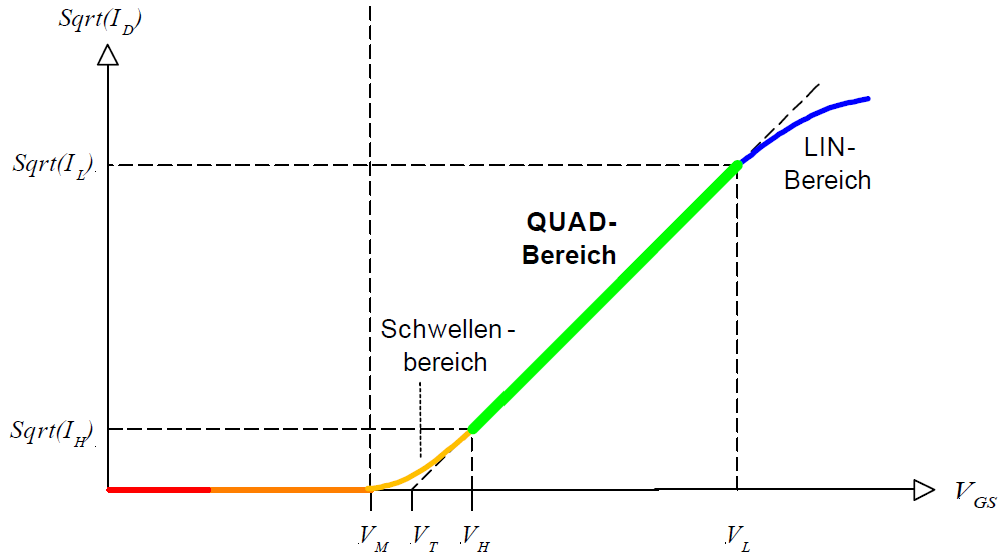
\includegraphics[width=1\linewidth]{Transferkennline_Sqrt.png}
\end{minipage}\newpage
\begin{minipage}{0.8\linewidth}
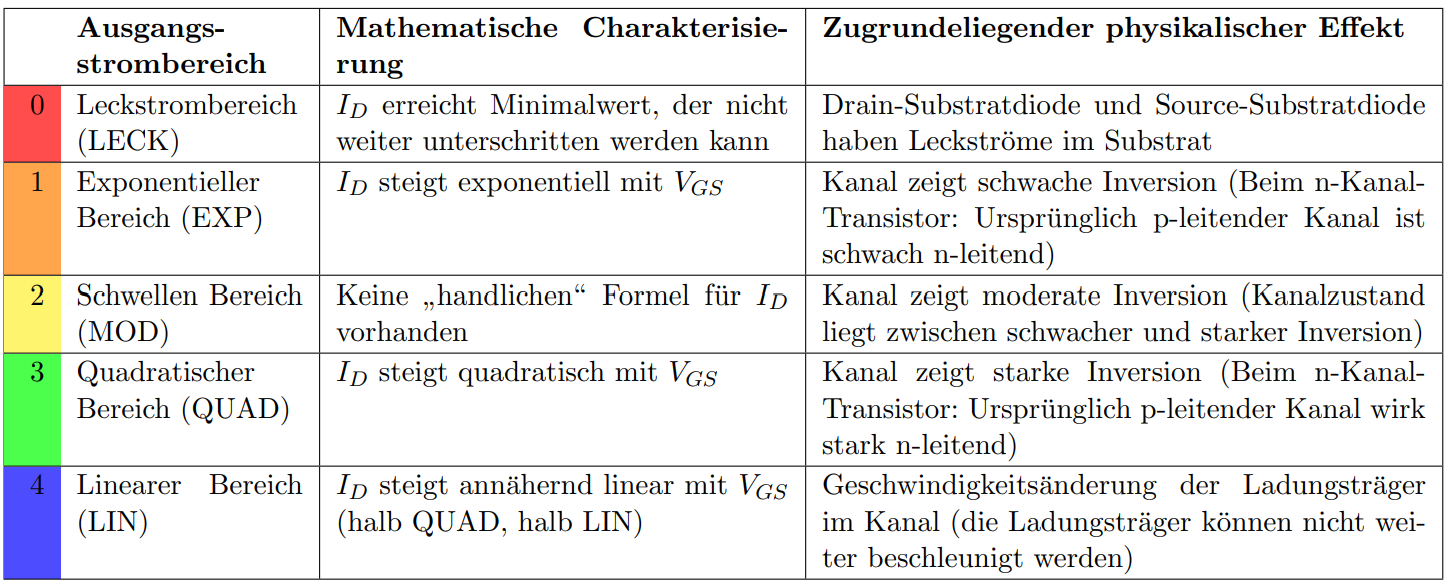
\includegraphics[width=1\linewidth]{Ausgangsstrombereiech.png}
\end{minipage}%
\begin{minipage}{0.2\linewidth}
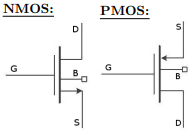
\includegraphics[angle=90, width=0.8\linewidth]{Selbstsperrend MOS-Transistor.png}
\end{minipage}
\textbf{Bulk-Anschluss}\\
Wenn der Bulk-Anschluss nicht gezeichnet ist, gilt die Konvention, dass der Bulk des n-Transistors immer mit $V_{SS}$ und der des p-Transistors immer mit $V_{\rm DD}$ verbunden ist. Wenn dies nicht der Fall ist dann steigt/sinkt die Schwellspannung $V_T$. Siehe Kap. 3.6.
\subsection{Bestimmung Arbeitsbereich}
\begin{enumerate}[noitemsep,topsep=0pt]
    \item Bestimmung ob in WEAK oder STRONG Inversion?
    \item Gesättigt/ Ungesättigt? (Für p-kanal gleiche Formel mit Betrag)
\end{enumerate}
\resizebox{1.0\columnwidth}{!}{%
\renewcommand{\arraystretch}{1.2}
\begin{tabular}{|l|l|l|}
\hline
\multicolumn{1}{|l|}{\textbf{Ausgangsstrom}} & \multicolumn{2}{c|}{Ausgangsspannungsbereich($V_{\rm DS}$-Bereich)}  \\
\multicolumn{1}{|l|}{($I_D-,V_{\rm GS}$-Bereich)}   & \multicolumn{1}{c|}{Transistor ungesättigt ($|V_{\rm DS}| < |V_{DS,sat}|$)}  & \multicolumn{1}{c|}{Transistor gesättigt ($|V_{\rm DS}| > |V_{DS,sat}|$)} \\
\hline
\multicolumn{3}{|c|}{\textbf{n-kanal Transistor}}  \\
\hline
\makecell[l]{\textbf{Weak inversion}\\$V_{DS,sat} \approx130mV$\\$V_{\rm GS}<V_M\hspace{3pt};\hspace{3pt}I_D<\frac{W}{L}I_M'$} & \makecell[l]{$I_D = I_M e^{\frac{V_{\rm GS}-V_M}{n_M V_{temp}}}(1-e^{\frac{-V_{\rm DS}}{V_{temp}}})$\textcolor{blue}{$(1+\lambda V_{\rm DS})$}} & \makecell[l]{$I_D = I_M e^{\frac{V_{\rm GS}-V_M}{n_M V_{temp}}}$\textcolor{blue}{$(1+\lambda V_{\rm DS})$}} \\
\hline
\makecell[l]{\textbf{Strong inversion}\\$V_{DS,sat} = V_{\rm GS}-V_T$\\$V_{\rm GS}>V_H\hspace{3pt};\hspace{3pt}I_D>\frac{W}{L}I_H'$} & \makecell[l]{$I_D = \textcolor{brown}{B}[(V_{\rm GS}-V_T)V_{\rm DS}-\frac{V_{\rm DS}^2}{2}]$\textcolor{blue}{$(1+\lambda V_{\rm DS})$}} & \makecell[l]{$I_D = \frac{\mu C_{\rm ox}}{2}\frac{W}{L}(V_{\rm GS}-V_T)^2$\textcolor{blue}{$(1+\lambda V_{\rm DS})$}}\\
\hline
\multicolumn{3}{|c|}{\textbf{p-kanal Transistor}}  \\
\hline
\makecell[l]{\textbf{Weak inversion}\\$|V_{DS,sat}| \approx 130mV$\\$|V_{\rm GS}|<|V_M|\hspace{3pt};\hspace{3pt}|I_D|<\frac{W}{L}|I_M'|$} & \makecell[l]{$I_D = I_M e^{-\frac{V_{\rm GS}-V_M}{n_M V_{temp}}}(1-e^{\frac{-V_{\rm DS}}{V_{temp}}})$\textcolor{blue}{$(1-\lambda V_{\rm DS})$}} & \makecell[l]{$I_D = I_M e^{-\frac{V_{\rm GS}-V_M}{n_M V_{temp}}}$\textcolor{blue}{$(1-\lambda V_{\rm DS})$}} \\
\hline
\makecell[l]{\textbf{Strong inversion}\\$|V_{DS,sat}| = |V_{\rm GS}|-|V_T|$\\$|V_{\rm GS}|>|V_H|\hspace{3pt};\hspace{3pt}|I_D|>\frac{W}{L}|I_H'|$} & \makecell[l]{$I_D = -\textcolor{brown}{B}[(V_{\rm GS}-V_T)V_{\rm DS}-\frac{V_{\rm DS}^2}{2}]$\textcolor{blue}{$(1-\lambda V_{\rm DS})$}} & \makecell[l]{$I_D = -\frac{\mu C_{\rm ox}}{2}\frac{W}{L}(V_{\rm GS}-V_T)^2$\textcolor{blue}{$(1-\lambda V_{\rm DS})$}} \\
\hline
\end{tabular}}\vspace{5pt}\\
Wird die Kanallängenmodulation vernachlässigt, so kann der \textcolor{blue}{$(1+\lambda V_{\rm DS})$} Term weggelassen werden.
\subsection{Kleinsignal Ersatzschaltung}
\begin{minipage}{0.5\linewidth}
\textbf{DC-Ersatzschaltung (Arbeitsspunkt definieren)}
    \begin{itemize}[noitemsep,topsep=0pt]
        \item AC-Spannungsquellen durch Kurzschluss ersetzen (AC-Quellen mit DC Offset zu DC-Quellen umzeichnen).
        \item AC-Stomquellen entfernen (Leerlauf)
        (AC-Quellen mit DC Strom zu DC-Quellen umzeichnen).
        \item Induktivitäten durch Kurzschluss ersetzen.
        \item Kapazitäten entfernen (Leerlauf)
    \end{itemize}
\end{minipage}%
\begin{minipage}{0.5\linewidth}
\textbf{Kleinsignal-Ersatzschaltung (AC)}
    \begin{itemize}[noitemsep,topsep=0pt]
        \item DC-Spannungsquellen kurzschliessen
        \item DC-Stromquellen entferen (Leerlauf)
        \item Nicht Lineare Bauteile durch ihre Kleinsignal-ersatzschaltungen ersetzen.
        \item ''Grosse'' Kondensatoren kurzschliessen
        \item ''Grosse'' Induktivitäten entfernen (Leerlauf)
    \end{itemize}
\end{minipage}\vspace{5pt}
\begin{tabular}{| l | l | l | l |}
    \hline
    Widerstandsbetrieb   & Stromquelllenbetrieb          & Hochfrequnez Ersatzschaltung \\
    (ungesättigt)        & (gesättigt, mit Body-Effekt)  & integrierter MOS-Transistor \\
    \hline
     & Pi-Ersatzschaltung  & \\
    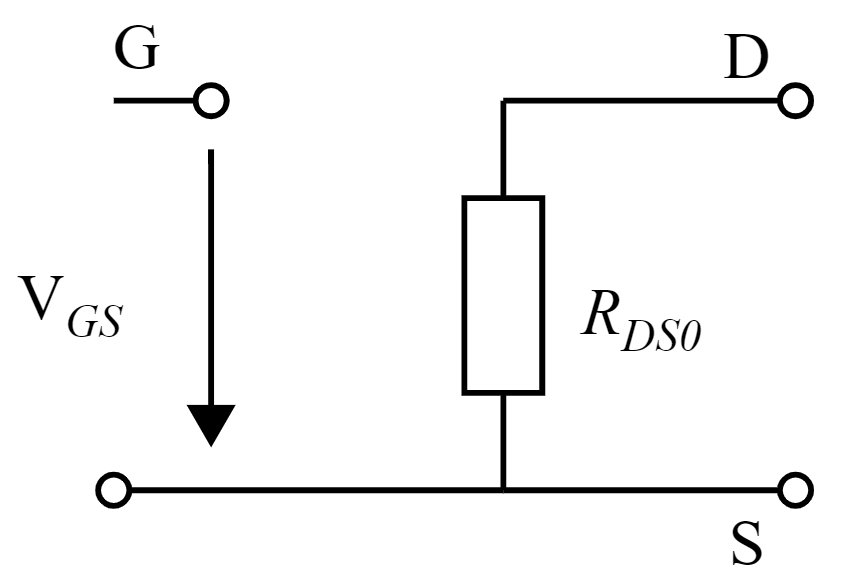
\includegraphics[width=0.2\linewidth]{Widerstandsbetrieb_Schaltung.png} & 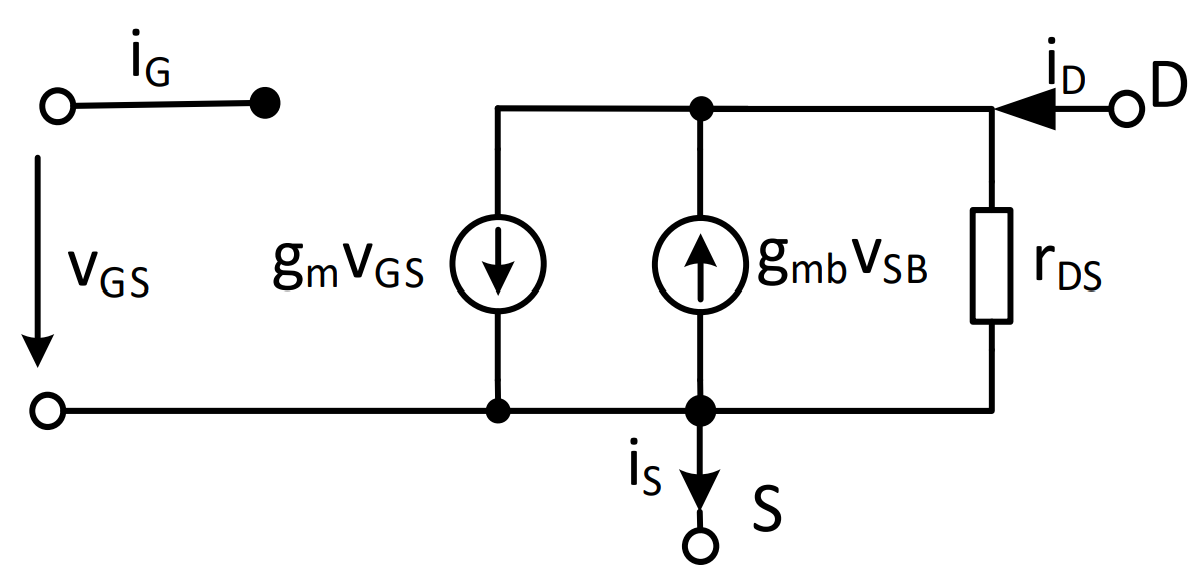
\includegraphics[width=0.3\linewidth]{PI_Niederfrequnz_Kleinsignal.png}  & 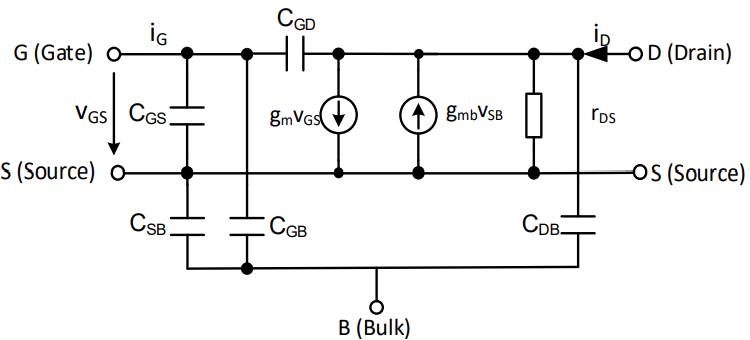
\includegraphics[width=0.3\linewidth]{Hochfrequnzbetrieb_Schaltung.png} \\
    \hline
\end{tabular}
\subsection{Kleinsignal Parameter}
\resizebox{1.0\columnwidth}{!}{%
\renewcommand{\arraystretch}{1.5}
\begin{tabular}{| l | l | l |}
    \hline
        & Transistor  ungesättigt (Widerstand) & Transistor gesättigt (Stromquelle)  \\
    \hline
    Weak Inversion      & $r_{DS0} = \frac{d V_{\rm DS}}{d I_D}|_{V_{\rm DS}=0} = \frac{V_{temp}}{I_{D\infty}}$     & \\
    EXP-Bereich         & $g_o = \frac{d I_D}{d V_{\rm DS}} = \frac{I_{D\infty - I_D}}{V_{temp}}$               & $g_o = \frac{1}{r_{\rm DS}} = \frac{d I_D}{d V_{\rm DS}} = \frac{I_D}{V_E + V_{\rm DS}}= \textcolor{blue}{\frac{I_D}{\frac{1}{\lambda}+ V_{\rm DS}}}$ \\
                        & $g_m$ wird nicht benötigt                                                         & $g_m = \frac{d I_D}{d V_{\rm GS}} = \frac{I_D}{n_M V_{temp}}$ \\
    \hline
    Strong Inversion    & $r_{DS0} = \frac{d V_{\rm DS}}{d I_D}|_{V_{\rm DS}=0} = \frac{1}{\mu C_{\rm ox}\cdot\frac{W}{L}(V_{\rm GS}-V_T)}$ & \\
    QUAD-Bereich        & $g_o = \frac{d I_D}{d V_{\rm DS}} = \mu C_{\rm ox}\cdot \frac{W}{L}(V_{\rm GS}-V_T - V_{\rm DS})$ & $g_o = \frac{1}{r_{\rm DS}} =\frac{d I_D}{d V_{\rm DS}} = \frac{I_D}{V_E + V_{\rm DS}}= \textcolor{blue}{\frac{I_D}{\frac{1}{\lambda}+ V_{\rm DS}}}$ \\
                        & $g_m$ wird nicht benötigt & $g_m = \frac{d I_D}{d V_{\rm GS}} = \mu C_{\rm ox}\cdot \frac{W}{L}(V_{\rm GS}-V_T) = \sqrt{2\mu C_{\rm ox}\frac{W}{L}I_D}$ \\
                        & $g_{\rm mb}$ wird nicht benötigt & $g_{\rm mb} = \frac{d I_D}{d V_{\rm SB}} = -g_m (n_M - 1)$ mit  \\
                        & & $n_M = 1 + \frac{\gamma}{2\sqrt{V_{\rm SB}+\Phi_0}}\approx 1.5-1.8$(bei $V_{\rm SB}$ = 0)\\
    \hline
\end{tabular}}
Dieselben Formel gelten auch für p-kanal Transistoren, wenn mit Beträgen gerechnet wird!
\subsection{Parameter}
\begin{tabular}{| l | l | l |}
    \hline
    $V_{DS,sat}$    & Sättigungsspannung    & Im EXP-Bereich: $V_{DS,sat} = -5 V_{temp}$\\
                    &                       & Im QUAD-Bereich: $V_{DS,sat} = V_{\rm GS} - V_T$\\
    \hline
    $V_T$           & Schwellenspannung     & Typisch 0.6V beim n-Kanal, resp.$-0.6V$ beim p-Kanal.\\
                    &                       & $V_T$ ist stark von der Source-Bulk Spannung abhängig (Body-Effekt):\\
                    &                       & $V_T = V_T0 \pm \Delta V_T$ mit $\Delta V_T = \gamma(\sqrt{V_{\rm SB}\pm 2\Phi_F}-\sqrt{2\Phi_F})$\hspace{10pt}$\Phi_0 = 2\Phi_F$ \\ 
                    &                       & ($+$ für n-Kanal, $-$ für p-Kanal)\\
                    &                       & $\gamma_N \approx 0.6V\sqrt{V}$ bzw. $\gamma_P \approx 0\sqrt{V} (\sqrt{V}$ ist die Einheit von $\gamma$)\\
                    &                       & Handrechnung: $\gamma \approx\gamma_N \approx\gamma_P\approx 0.6\sqrt{V}$ \\
    \hline
    $\Phi_t$        & Temperaturspannung    & $\Phi_t = V_{temp} = k\cdot T/e = 86.2\mu V/(K T)$ \\
                    &                       & somit ist $\Phi_t = 25.9 mV$ bei $T = 300$ K bzw. 27°C, $e = 1.6\cdot 10^{-19}C$\\
    \hline
    $I_M$           & Drainstrom            & Drainstrom an der Grenze zwischen schwacher und moderater Inversion. \\
                    &                       & \colorbox{lime}{$I_M = \frac{W}{L}\cdot I'_M$} \\
                    &                       & $I'_M$ ist der spezifische Drainstrom an der Grenze. \\
    \hline
    $n_M$           & Unterschwellen-       & Der Faktor $n_M$ ist von der Source-Bulk Spannung $V_{\rm SB}$ abhängig:\\
                    & Neigungsfaktor        & $n_M = 1 + \frac{\gamma}{2\sqrt{V_{\rm SB}+\Phi_0}}$\\
                    &                       & mit $\Phi_0 = 2\Phi_F\approx0.6$V. Für $V_{\rm SB}$ = 0V erhalten wir $n_M = 1.39.$ \\
                    &                       & Häufig wird ein Wert von $n_M\approx1.5$ angegeben \\
    \hline
    $a_E$           & Early-Faktor          & \textcolor{gray}{(gemäss Technologieparametern)} \\
    \hline
    $V_E$           & Early-Spannung        & $V_E \approx a_E \cdot L$ \hspace{10pt} $V_E$ ist immer positiv \\
    \hline
    $\lambda$       & Kanallängen-          & inverser Wert der Early-Spannung \\
                    & Modulationsfaktor     & $\lambda = \frac{1}{V_E + V_{DS,sat}}\approx\frac{1}{V_E}\approx\frac{1}{a_E \cdot L}$\\
                    &                       & Bei der Handrechnung wird der MOS-Transistor meistens mit \textcolor{blue}{$\lambda=0$} idealisiert\\
    \hline
    $\beta$,B,$\mu C_{\rm ox}$       & Transkonduktanz       & Steilheit, Verstärkungsfaktor. Dieser Faktor ist im gesättigten ($\beta$) und \\
                    &                       & ungesättigten Bereich (B) grundsätzlich verschieden. \\
                    &                       & Es gilt: $\beta = \frac{W}{L}\beta_0$ bzw. $B = \frac{W}{L}B_0; B_0\approx \beta_0 = \mu C''_{ox}$ \\
    \hline
    $g_m$           & Transkonduktanz       & Steilheit oder Gate-Steilheit. Beschreibt den Zusammenhang zwischen \\
                    &                       & $I_{DS}$ und $V_{\rm GS}$. Mass für die Verstärkung. (Siehe Tabelle Kleinsignalparameter) \\
    \hline
    $g_{\rm mb}$        & Body-Transkonduktanz  & Beschreibt die Wirkung des Body-Effekts. Nur im gesättigtem \\
                    &                       & Stromquellenbetrieb von Bedeutung. \\
    \hline
    $g_o$           & Ausgangsleitwert      & $g_o = 1/(r_{\rm DS}) = I_D/(V_E + V_{\rm DS})$\\
    \hline
    $r_{\rm DS}$        & Ausgangswiderstand    & $r_{\rm DS} = \frac{1}{g_o}\approx\frac{\Delta V_{\rm DS}}{\Delta I_D}$ oder $r_{\rm DS} = \frac{V_E + V_{\rm DS}}{I_{D,real}}\approx\frac{V_E}{I_D}$\\
                    &                       & $V_E, V_{\rm DS}, I_{D,real}$ immer im Betrag! \\
    \hline
    $r_{DS0}$       & Eingangswiderstand    & Kleinstmöglicher Ausgangswiderstand (bei $V_{\rm DS} = 0V$), Widerstandsbetrieb bei\\
                    &                       & $V_{\rm DS} \leq V_{DS,sat}$ \\
    \hline
    $r_s$           & innerer                & \\
                    & Sourcewiderstand       & $r_s = 1/g_m = 1 / \sqrt{2\mu C_{\rm ox} I_D}$\\
    \hline
    \end{tabular}
\section{Verstärker Grundschaltungen }
\renewcommand{\arraystretch}{1.3}
\begin{tabular}{|l|l|l|l|}
    \hline
    Typ             &  \textbf{Source-Schaltung} & \textbf{Gate-Schaltung}           & \textbf{Drain-Schaltung} \\
    \hline
    Schaltschema    & 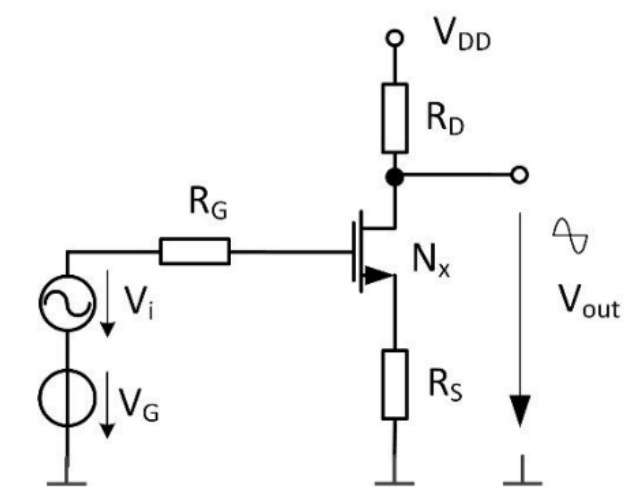
\includegraphics[width=0.2\linewidth]{Source_Schaltung.png} & 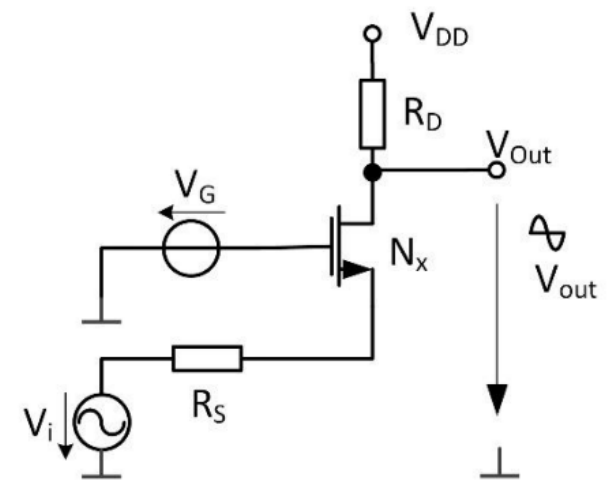
\includegraphics[width=0.2\linewidth]{Gate_Schaltung.png} & 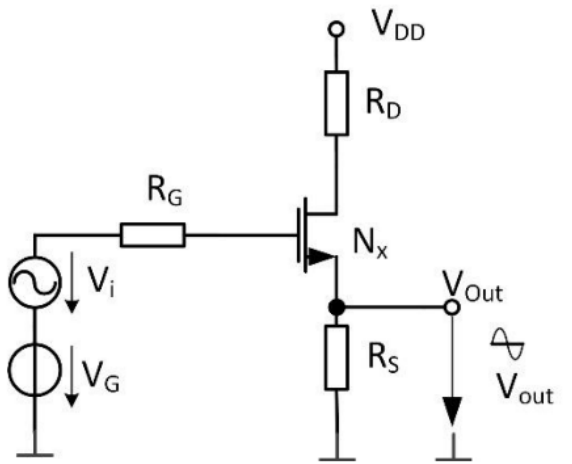
\includegraphics[width=0.2\linewidth]{Drain_Schaltung.png} \\
    \hline
    Eigenschaft     &  Invertierender Verstärker & Nichtinvertierender Verstärker    & Nichtinvertierender Verstärker \\
    \hline
    Anwendung       & Verstärkung tiefe bis mittlere & Verstärker hohe Frequenzen    & Spannungsfolger/ Impedanz- \\
                    & Frequenzen                     & (HF-Verstärker)               & wandler / Leistungstreiber \\
    \hline
    $R_{in}/R_{out}$ & gross/gross                   & klein/gross                   & gross/klein \\
    \hline
    Verstärkung     &  $a=\frac{V_{out}}{V_{in}}= -\frac{R_D}{R_S + \frac{1}{g_m}+(R_D+R_S)\frac{g_o}{g_m}}$        & $a=\frac{V_{out}}{V_{in}}= \frac{R_D (1+\frac{g_o}{g_m})}{R_S + \frac{1}{g_m}+(R_D+R_S)\frac{g_o}{g_m}}$              & $a=\frac{V_{out}}{V_{in}}= \frac{R_S}{R_S + \frac{1}{g_m}+(R_D+R_S)\frac{g_o}{g_m}}$ \\
    Spezialfälle    & Bei $1/g_m, R_D<<1/g_o$:     & Bei $1/g_m, R_D<<1/g_o$:       & Bei $R_S,R_D<<1/g_o$: \\
                    & $a \approx -\frac{R_D}{R_S+\frac{1}{g_m}}$    & $a \approx \frac{R_D}{R_S+\frac{1}{g_m}}$     & $a \approx \frac{R_S}{R_S+\frac{1}{g_m}}$ \\
                    & Bei $R_S$=0:                 & Bei $R_S$=0:                   & Idealer Source-Folger: $a\approx1$ \\
                    & $a\approx -g_m(R_D||r_{\rm DS})$  & $a\approx g_m(R_D||r_{\rm DS})(1+\frac{g_o}{g_m})$       & $(1/g_m<<R_S<<1/g_o)$ \\
    \hline
    \multicolumn{4}{|l|}{$g_m = \frac{1}{r_s}$ \hspace{15pt} $g_o = \frac{1}{r_{\rm DS}}= \frac{I_D}{V_E+V_{\rm DS}}\approx\frac{I_D}{V_E}$ (Näherung für $V_E>>V_{\rm DS}$) \hspace{10pt} $V_E = a_E\cdot L (V_E=5$V...100V, Kanallängenabh.)} \\
    \hline
\end{tabular}\vspace{5pt}\\
\textbf{Innenwiderstände}\\
\renewcommand{\arraystretch}{1}
\begin{tabular}{|l|l|l|}
    \hline
    \textbf{Source}                 & \textbf{Gate}                     &\textbf{Drain} \\
    \hline
    Näherung für $1/g_o>>R_D$       & $r_{iG}\rightarrow\infty$     & Näherung für $1/g_o>>R_D$ \\
    $r_{iS}\approx r_s||r_{\rm DS}=\frac{1}{g_m+g_o}$       &  $r_{iG}=100M\Omega ...10 G\Omega$     & $r_{iD}\approx r_{\rm DS}(1+\frac{R_S}{r_s})=\frac{1}{g_o}(1+g_mR_s)$ \\
    Näherung für $R_S = 0$                              &           & Näherung für $g_m, 1/R_D>>g_o$ \\
    $r_{iS}\approx r_S = \frac{1}{g_m}$                 &           & $r_{iD}\approx r_{\rm DS} = \frac{1}{g_o}$ \\
    \hline
\end{tabular}
\section{MOS-Diode}
\begin{tabular}{|l|l|l|l|l|l|}
    \hline
    \multicolumn{2}{|l|}{\textbf{Reale Diode:}} & \multicolumn{4}{l|}{\textbf{MOS-Diode:}} \\
    \hline
    Symbol      & Kennline      & N-MOS Diode       & P-MOS Diode       & Kennline      & KS-Ersatzschaltung \\
    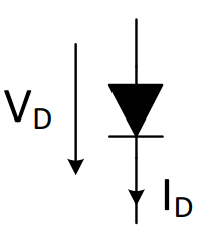
\includegraphics[width=0.11\linewidth]{Reale Diode.png} & 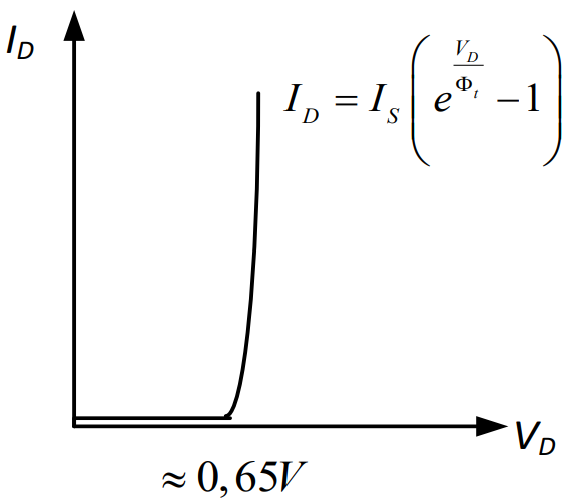
\includegraphics[width=0.14\linewidth]{Reale Diode_Kennline.png} &
    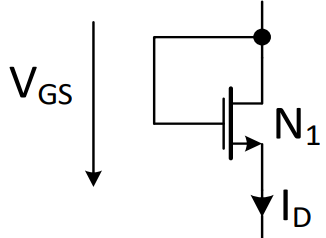
\includegraphics[width=0.13\linewidth]{N-MOS Diode.png} & 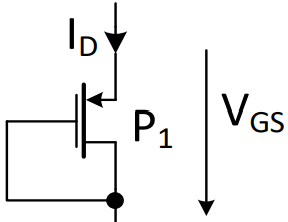
\includegraphics[width=0.13\linewidth]{P-MOS Diode.png} & 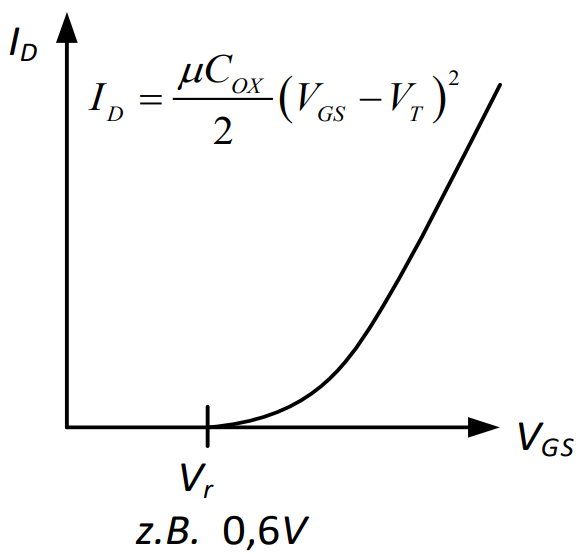
\includegraphics[width=0.14\linewidth]{MOS-Diode_Kennline.png} & 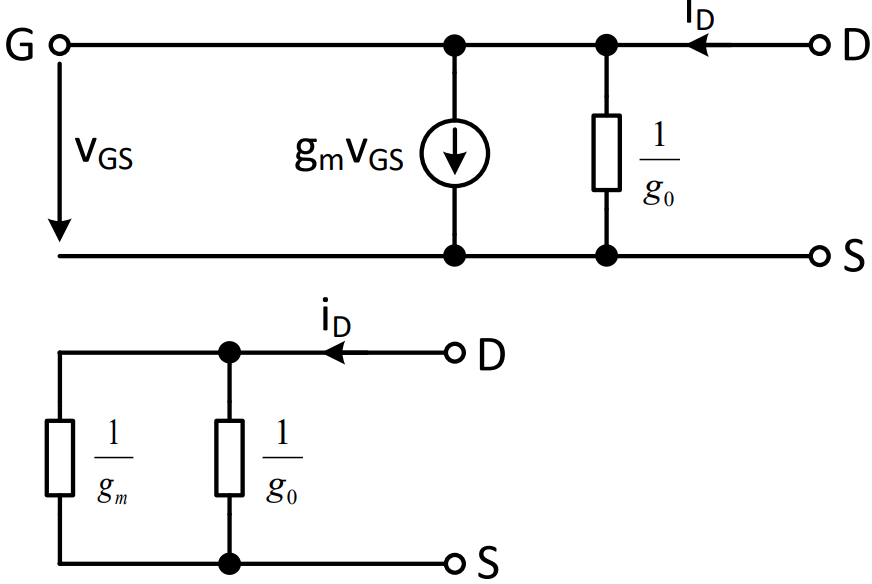
\includegraphics[width=0.2\linewidth]{MOS-Diode_KS.png} \\
    \hline
\end{tabular}\vspace{5pt}\\
\renewcommand{\arraystretch}{1.2}
\begin{tabular}{|l|l|}
    \hline
    Arbeitspunktstrom einer MOS-Diode mit Widerstandslast $R_D$ & $I_D = \frac{\mu C_{\rm ox}}{2}\frac{W}{L}(V_{\rm GS}-V_T)^2\textcolor{blue}{(1+\lambda V_{\rm DS})}= \frac{V^+-V_{\rm GS}}{R_D}$ \\
    \hline
    $V_{\rm DS}$ einer MOS-Diode bei gegebenem Strom                & $V_{\rm DS} = V_T + \sqrt{\frac{2 I_D}{\mu C_{\rm ox}\frac{W}{L} \textcolor{blue}{(1+\lambda V_{\rm DS})}}}\approx V_T + \sqrt{\frac{2 I_D}{\mu C_{\rm ox}\frac{W}{L}}}$ \\
    \hline
    Innenwiderstand der MOS-Diode                               & $r_{DM} = \frac{V_{\rm GS}}{I_D} = \frac{1}{g_m+g_o} \approx \frac{1}{g_m}$ \\
    \hline
    Im quadratischen Bereich gilt                               & $g_m = \mu C_{\rm ox}\frac{W}{L} (V_{\rm GS}-V_T) = \sqrt{2\mu C_{\rm ox}\frac{W}{L} I_D}$ \\
    \hline
\end{tabular}\vspace{5pt}\\
Bei der leitenden MOS-Diode ist der Transistor \textbf{immer gesättigt}, weil $V_{\rm DS}>V_{DS,sat} = (V_{\rm GS}-V_T)$ jederzeit erfüllt ist. Auch kann die MOS-Diode in der Strong, Moderate und Weak Inversion tätig sein. \\
\textbf{MOS-Dioden als Spannungsteiler}\\
\renewcommand{\arraystretch}{1}
\begin{tabular}{|l|l|l|l|}
    \hline
    \textbf{Mit Bodyeffekt}     & \textbf{Ohne Bodyeffekt}      & \multicolumn{2}{l|}{\textbf{Mehrfach Spannungsteiler}} \\
    \hline
    $V_{SB1} = 0, V{SB2} = G_{GS1}$ & $V_{SB1} = 0, V{SB2} = 0$ daher kein  & Lokales Substrat, $V_{Ti}$ für        & Gemeinsames Substrat, unter- \\
    daher Body-Effekt und           & Body-Effekt. Es gelten die            & alle gleich $\rightarrow$ gleiche     & schiedliche $V_{Ti} \rightarrow$ unterschied- \\
    $V_{T2}>V_{T1}$                 & Nominalwerte für $V_{T2},V_{T1}$      & Teilspannungen                        & liche Teilspannungen \\
    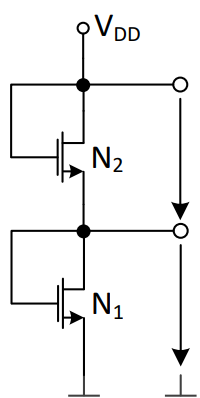
\includegraphics[width=0.08\linewidth]{Spannungsteiler_mit Body_Effekt.png}    & 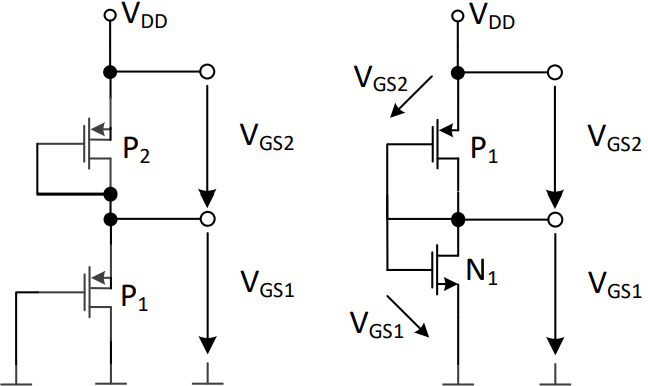
\includegraphics[width=0.22\linewidth]{Spannungsteiler_ohne Body_Effekt.png}  & 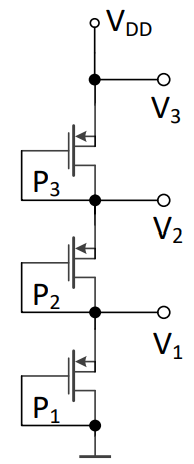
\includegraphics[angle=90,width=0.2\linewidth]{Mehrfach_Spannungsteiler_getrennte Substrate.png}   & 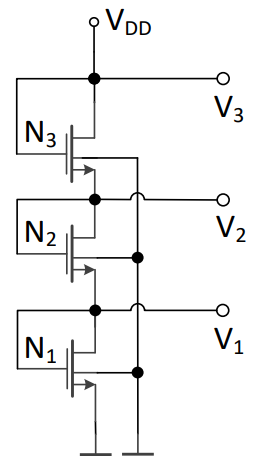
\includegraphics[angle=90, width=0.2\linewidth]{Mehrfach_Spannungsteiler_gemeinsame Substrate.png}\\
    \hline
\end{tabular}\vspace{5pt}\\
\textbf{Verhältnis:} $\frac{|V_{GS1}-V_{T1}|}{|V_{GS2}-V_{T2}|}= \sqrt{\frac{\beta_2}{\beta_1}}=\sqrt{\frac{(W/L)_2\beta_2}{(W/L)_1\beta_1}}\rightarrow \Bigl|\frac{V_{GS1}}{V_{GS2}}\Bigr| = \frac{V_{T1}\pm\sqrt{\frac{2I_D}{\beta_1}}}{V_{T2}\pm\sqrt{\frac{2I_D}{\beta_2}}}$ \hspace{20pt}($\beta = \mu C_{\rm ox} \frac{W}{L}$)
\section{MOS-Transistor als Stromquelle}
Die Drain-Source-Strecke des MOS-Transistors stellt im Sättigungsbereich eine gesteuerte Stromquelle dar, deren Ausgangswiderstand (Innenwiderstand am Drain) relativ hoch ist.\\
\begin{minipage}{0.5\linewidth}
\subsection{Strom einer MOS Stromquelle}
$I_D = \frac{\mu C_{\rm ox}}{2}\frac{W}{L}(V_{\rm GS}-V_T)^2\textcolor{blue}{(1+\lambda V_{\rm DS})}\approx\frac{\mu C_{\rm ox}}{2}\frac{W}{L}(V_{\rm GS}-V_T)^2$
\end{minipage}%
\begin{minipage}{0.5\linewidth}
\subsection{Sättigungsspannung}
\textbf{Bei strong Inversion:}\\ $V_{\rm DS} \geq V_{DS,sat} = V_{\rm GS} - V_T = \sqrt{\frac{2 I_D}{\mu C_{\rm ox}\frac{W}{L}}}$\vspace{5pt}\\
\textbf{Bei Weak Inversion:} $V_{\rm DS} \geq V_{DS,sat}\approx 130 mV$
\end{minipage}\vspace{5pt}\\
\begin{tabular}{|l|l|l|}
    \hline
    \textbf{Einfache Stromquelle mit und} & \textbf{Stromquelle mit Kaskode} & \textbf{Stromquelle mit geregelter} \\
    \textbf{ohne Source-Widerstand}         &                                  & \textbf{Kaskode} \\
    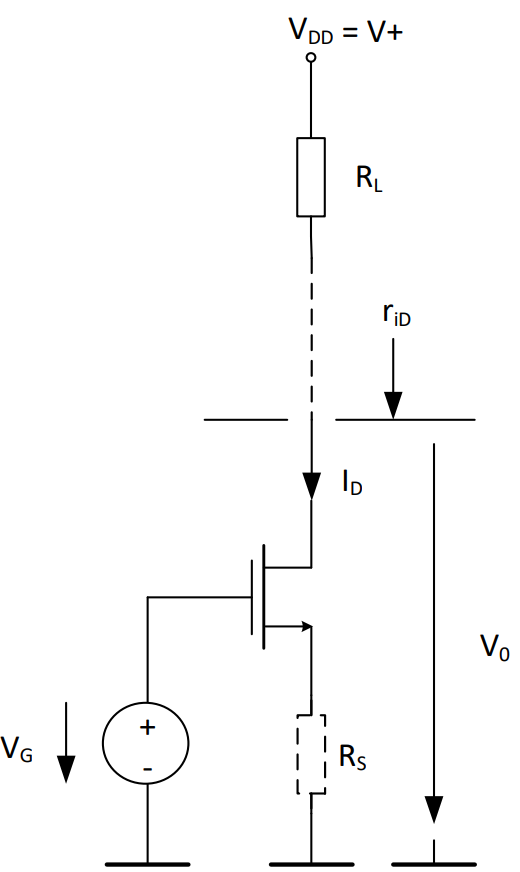
\includegraphics[width=0.15\linewidth]{Einfachste Stromquelle.png} & 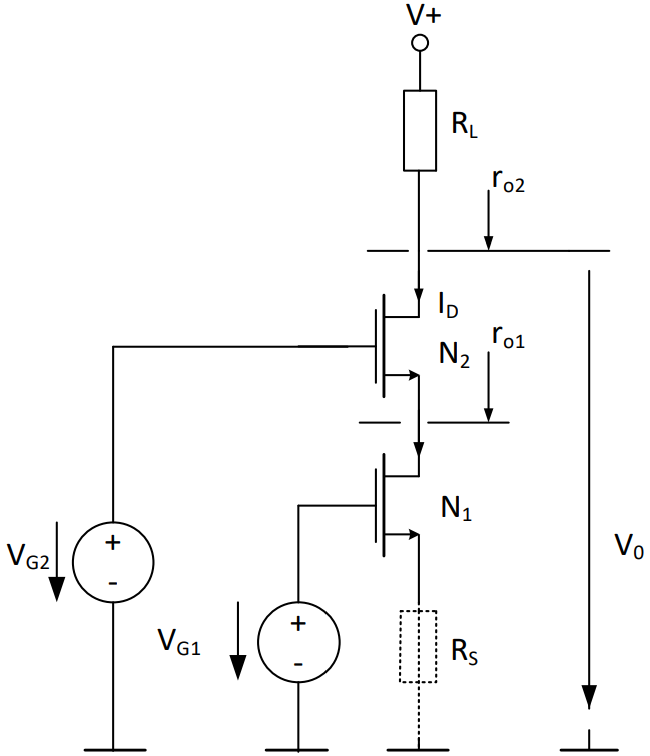
\includegraphics[width=0.2\linewidth]{Stromquelle mit Kaskode.png} & 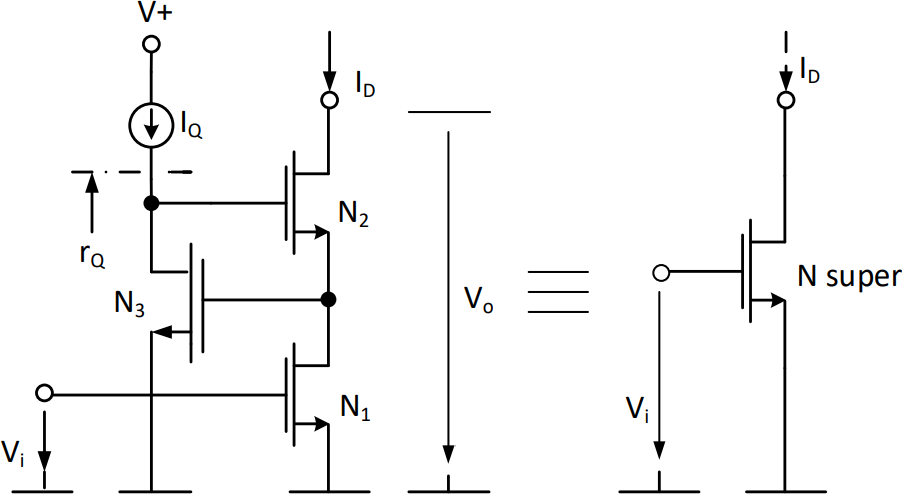
\includegraphics[width=0.3\linewidth]{Super Transistor.png} \\
    \hline
\end{tabular} \vspace{5pt}\\
\renewcommand{\arraystretch}{1.2}
\begin{tabular}{|l|l|l|}
    \hline
    \textbf{Konfiguration}  & \textbf{Ausgangswiderstand $r_0$}     & \textbf{min. Ausgangsspannung $V_{0,min}$} \\
    \hline
    Einfache Quelle      & $r_{out} = r_{iD} = r_{\rm DS} = \frac{1}{g_o}= \frac{V_E+V_{\rm DS}}{I_D}\approx\frac{V_E}{I_D}$ & $V_0 > V_{0,min} = V_{DS,sat}$ \\
    mit 1 Transistor     &  & \\
    \hline
    Stromquelle mit      & $r_{iD} = r_{\rm DS}\Bigl(1+g_m R_S+\frac{R_S}{r_{\rm DS}}\Bigr)$ & $V_0 > V_{0,min} = R_S I_D + V_{DS,sat}$ \\
    Source-Widerstand    & $= \frac{1}{g_o}(1+g_m R_S)+R_S$ & \\
    \hline
    Stromquelle mit      & $r_{out} = r_{o2}\approx g_{m2}\cdot r_{\rm DS}^2 = (g_m r_{\rm DS})r_{\rm DS}$ & $V_{0,min} = V_{G2}-V_{GS2}+V_{DS2,sat}$\\
    Kaskode              & $= \mu\cdot r_{\rm DS} = \frac{1}{g_{01}}\cdot\frac{g_{m2}}{g_{02}}$ & $V_{0,min} = V_{DS1,sat}+V_{DS2,sat}$ \\
        &   & (bei $V_{G2} = V_{DS1,sat} +V_{GS2})$ \\
    \hline
    Stromqulle mit       & $r_{out}\approx r_{DS1}\cdot g_{m2}r_{DS2}\cdot g_{m3}r_{DS3}$ & $V_{0,min} = 2 V_{DS,sat}$\\
    geregelter Kaskode   & $=\frac{1}{g_{01}}\cdot\frac{g_{m2}}{g_{02}}\cdot\frac{g_{m3}}{g_{03}}$ &  \\
        & & \\
    \hline
\end{tabular}\newpage
\section{MOS-Stromspiegel}
\begin{minipage}{0.33\linewidth}
\textbf{Stromspiegelverhältnis}\\
$n_m = \frac{I_{out}}{I_{in}} = \frac{(\frac{W}{L})_2}{(\frac{W}{L})_1}$\\
\\
\end{minipage}%
\begin{minipage}{0.33\linewidth}
\textbf{Berechnung Ausgangsstrom} \\
$I_{out} = I_{in}\cdot \frac{(\frac{W}{L})_2}{(\frac{W}{L})_1}$ (allgemein)\vspace{5pt}\\
$I_{out} = I_{in}\cdot \frac{W_{T2}}{W_{T1}}$ (wenn $L_{T2} = L_{T1}$)
\end{minipage}%
\begin{minipage}{0.33\linewidth}
\textbf{Impedanz}\\
Eingangsimpedanz (ideal): $r_{in}=0\Omega$\\
Ausgangsimpedanz (ideal): $r_{out}=\infty\Omega$\\
\end{minipage}\\
\begin{tabular}{|l|l|l|}
    \hline
    \textbf{Widlar-Stromspiegel} & \textbf{Wilson-Stromspiegel} & \makecell[l]{\textbf{verbesserter}\\ \textbf{Wilson-Stromspiegel}}\\
    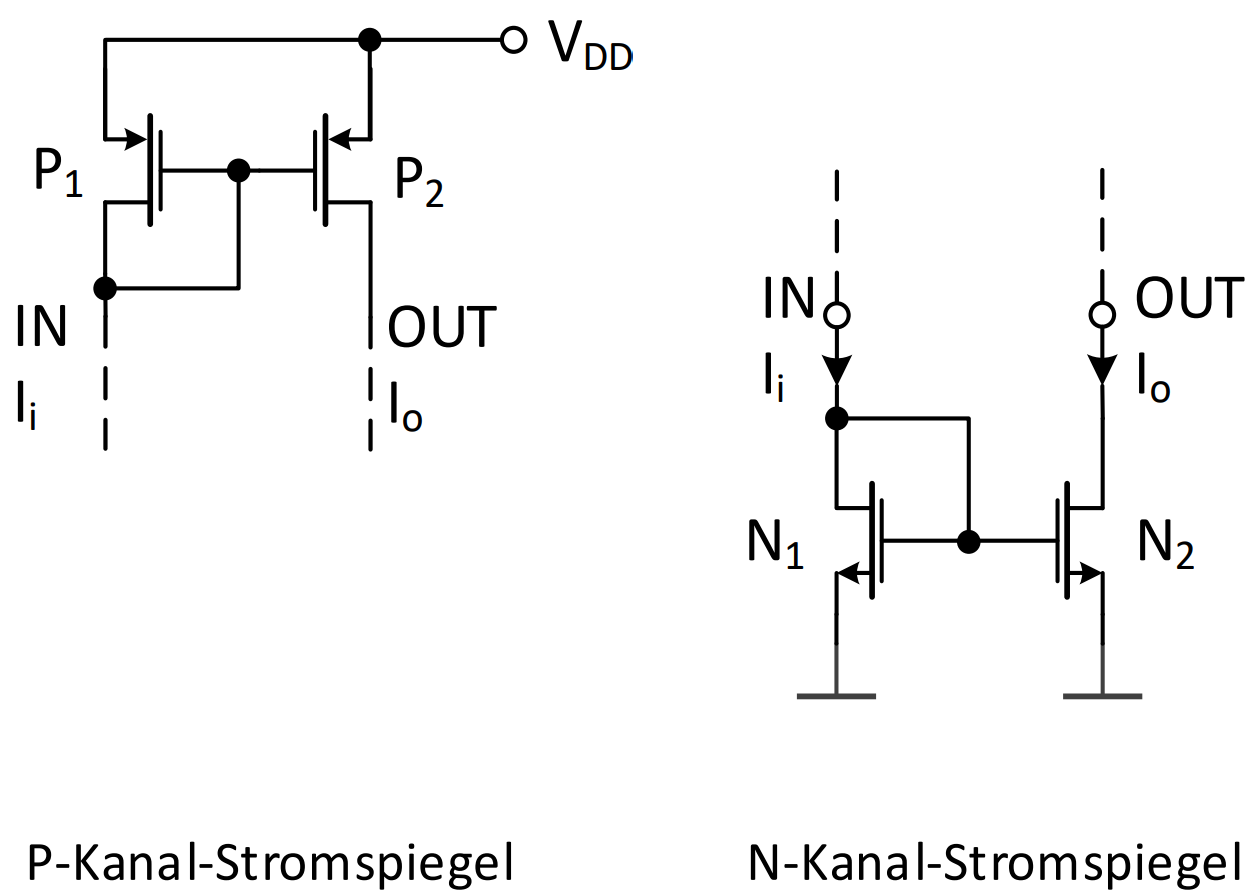
\includegraphics[width=7cm]{Widlar Stromspiegel.png} & 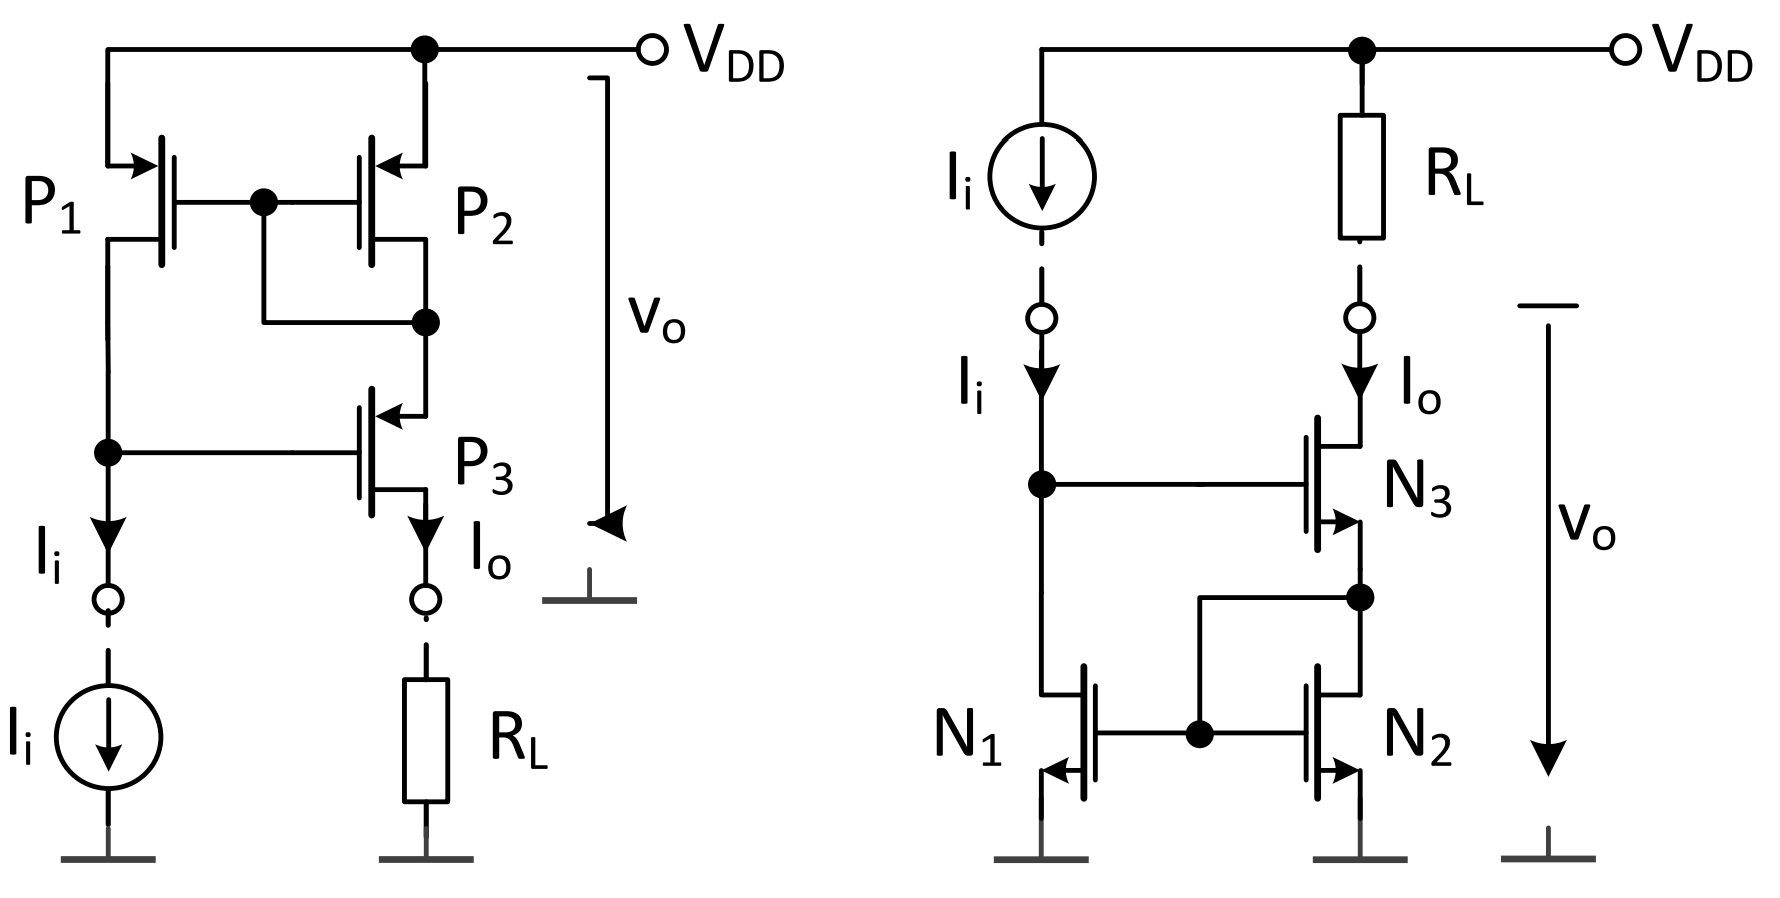
\includegraphics[width=7cm]{Wilson Stromspiegel.png}  & 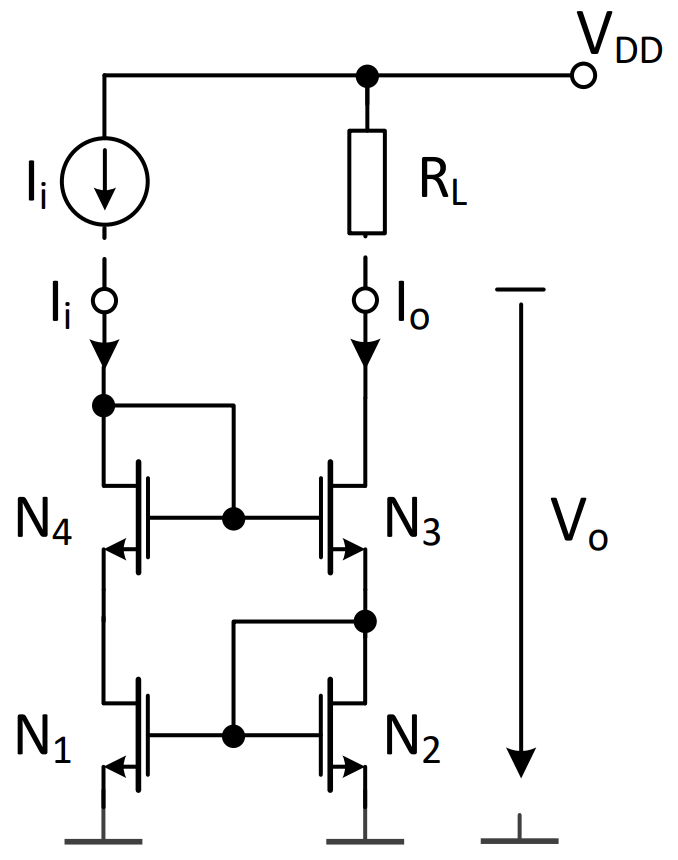
\includegraphics[width=4cm]{Verbesserter Wilson Stromspiegel.png}\\
    \hline
\end{tabular}\\
\begin{tabular}{|l|l|}
    \hline 
    \textbf{Kaskode}  & \textbf{geregelte Kaskode} \\
     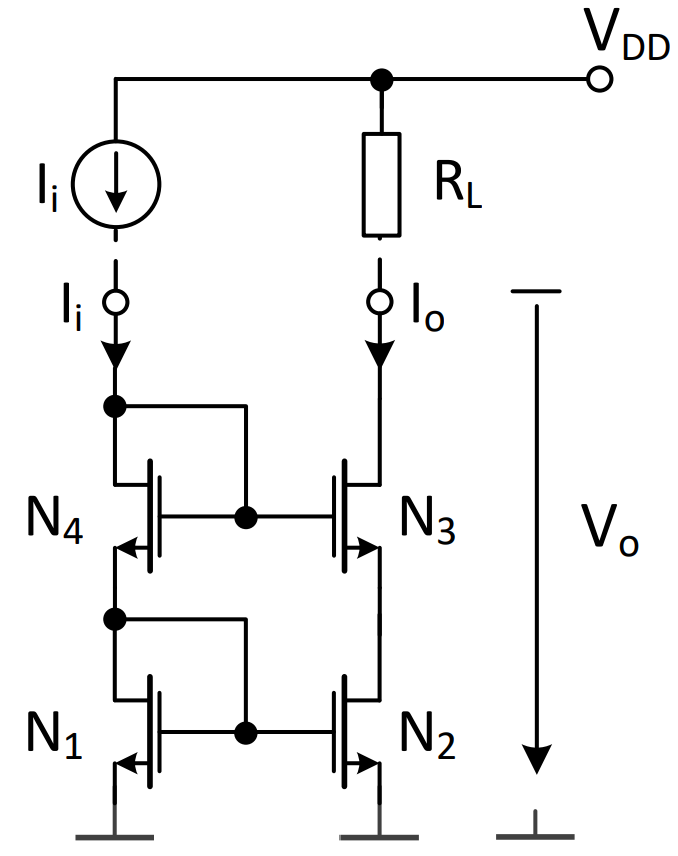
\includegraphics[width=4cm]{Kaskode Stromspiegel.png}  & 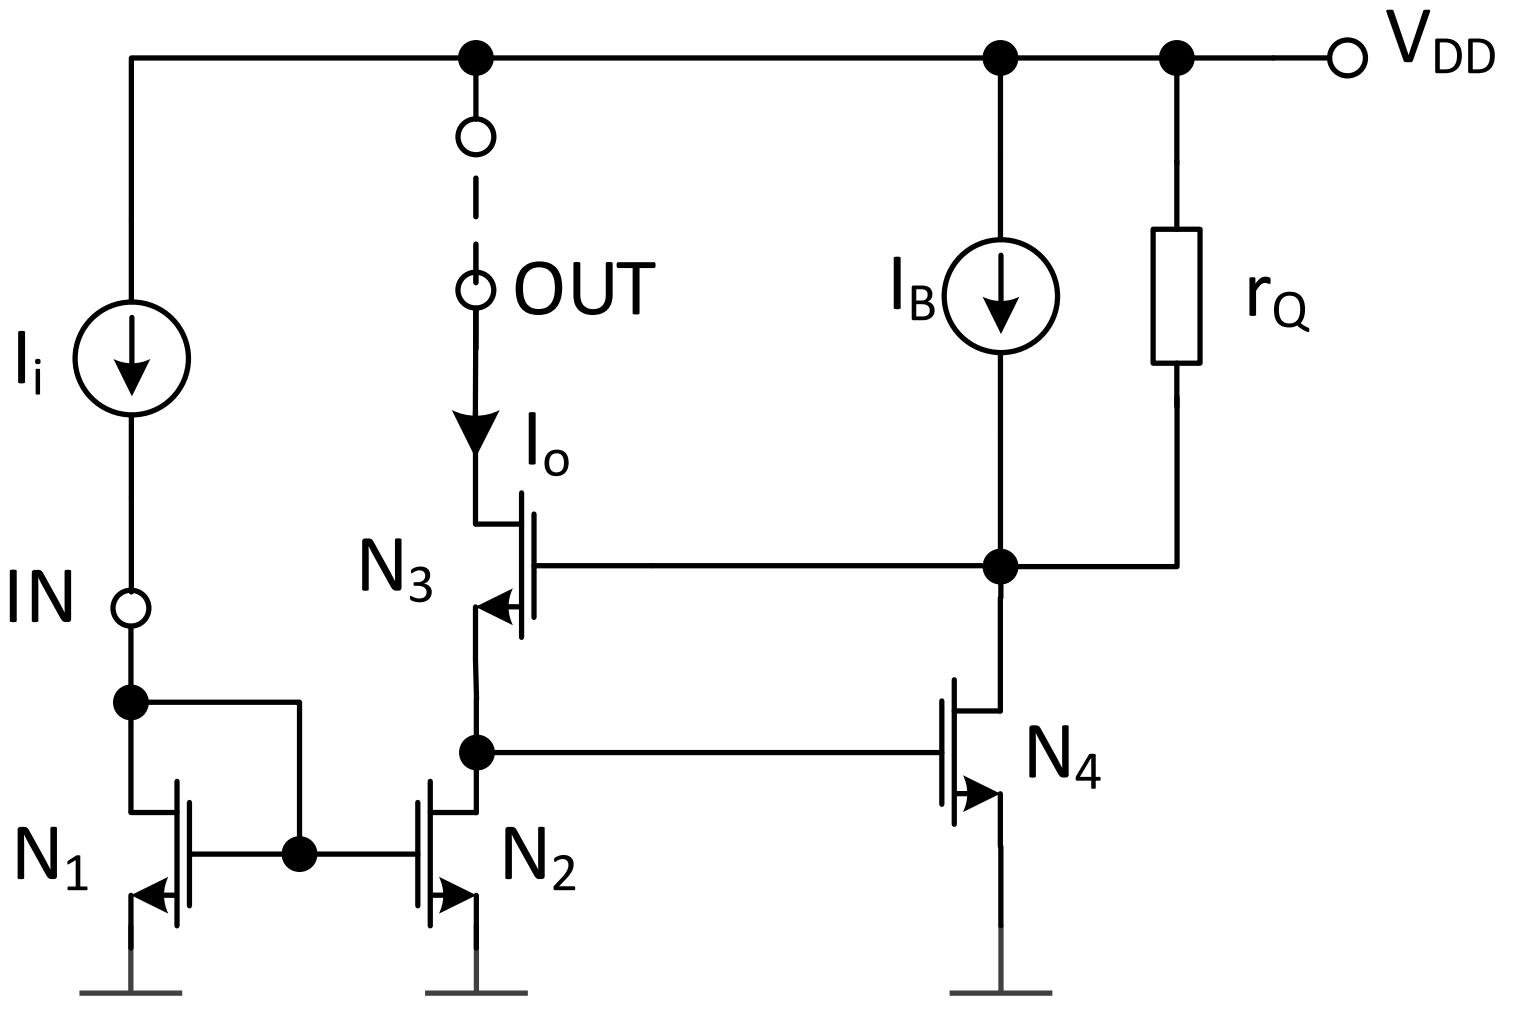
\includegraphics[width=7cm]{Geregelte Kaskode Stromspiegel.png}\\
    \hline 
\end{tabular}\\
\renewcommand{\arraystretch}{1.5}
\begin{tabular}{|l|l|l|l|l|}
    \hline 
    \textbf{Stromspiegeltyp} & \textbf{Genauigkeit} & $r_{out}$ & $V_I$ & $V_{O,min}$ \\
    \hline
    Widlar-Stromspiegel     & $+$     & $=\frac{1}{g_o}$                              & $\approx V_T + \sqrt{\frac{2 I_I}{\mu C_{\rm ox}\frac{W}{L}}}$    & $\approx \sqrt{\frac{2 I_0}{\mu C_{\rm ox}\frac{W}{L}}}$ \\
    \hline
    Wilson-Stromspiegel     & $+$     & $\approx\frac{1}{g_o}(2+\frac{g_m}{g_o})$     & $\approx 2V_T + 2\sqrt{\frac{2 I_I}{\mu C_{\rm ox}\frac{W}{L}}}$   & $\approx V_T + 2\sqrt{\frac{2 I_0}{\mu C_{\rm ox}\frac{W}{L}}}$ \\
    \hline
    Verbesserter Wilson     & $+ +$   & $\approx\frac{1}{g_o}(2+\frac{g_m}{g_o})$     & $\approx 2V_T + 2\sqrt{\frac{2 I_I}{\mu C_{\rm ox}\frac{W}{L}}}$   & $\approx V_T + 2\sqrt{\frac{2 I_0}{\mu C_{\rm ox}\frac{W}{L}}}$ \\
    \hline
    Kaskode-Stromspiegel    & $+ +$   & $\approx\frac{1}{g_o}(2+\frac{g_m}{g_o})$     & $\approx 2V_T + 2\sqrt{\frac{2 I_I}{\mu C_{\rm ox}\frac{W}{L}}}$   & $\approx V_T + 2\sqrt{\frac{2 I_0}{\mu C_{\rm ox}\frac{W}{L}}}$ \\
    \hline
    geregelte Kaskode       & $+ +$   & $\approx\frac{1}{g_o}(\frac{g_m}{g_o})^2$     & $\approx V_T + \sqrt{\frac{2 I_I}{\mu C_{\rm ox}\frac{W}{L}}}$    & $\approx2\sqrt{\frac{2 I_0}{\mu C_{\rm ox}\frac{W}{L}}}$ \\
    \hline
\end{tabular}\\
\textbf{Beeinflussung von Stromspiegelverhältnis mittels hinzufügen von Sourcewiderstand} \\
Strong Inversion: $R_S=\frac{1}{I_{D2}} \Bigl(\sqrt{\frac{2I_{D1}}{\beta_1}} - \sqrt{\frac{2I_{D2}}{\beta_2}}\Bigr)$ \hspace{20pt}($\beta = \mu C_{\rm ox} \frac{W}{L}$)\\
Weak Inversion: $R_S = \frac{1}{I_{D2}}\cdot n_M\cdot V_{temp} \cdot \ln(\frac{I_{D1}}{I_{D2}})$\\
\textbf{Serie/Parallelschaltung von Transistoren} \\
Bei der Serieschaltung von k identischen Transistoren mit dem Kanal-Seitenverhältnis (W/L) entsteht eine Schaltung, welche sich wie ein neuer Transistor mit dem Kanal-Seitenverhältnis (W/k$\cdot$L) verhält. \\
Bei der Parallelschaltung von n identischen Transistoren mit dem Kanal-Seitenverhältnis (W/L) entsteht quasi ein neuer Transistor mit dem Kanal-Seitenverhätnis (n$\cdot$W/L).\\
\begin{minipage}{0.5\linewidth}
    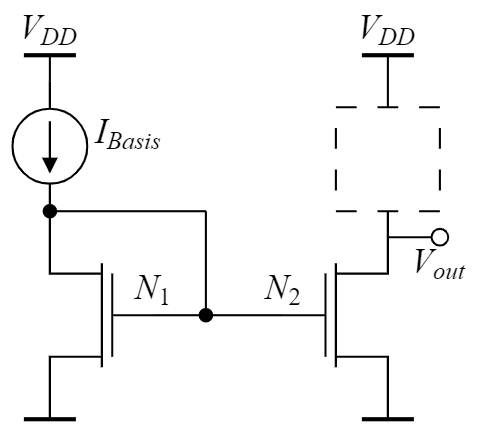
\includegraphics[width=3.5cm]{Stromspiegel_mitStromquelle_GS.png}\\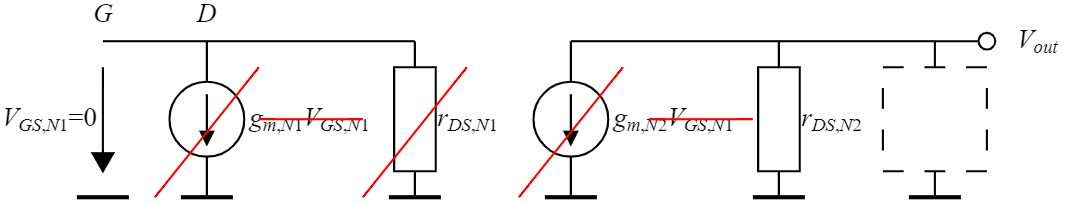
\includegraphics[width=8.5cm]{Stromspiegel_mitStromquelle_KS.png}
\end{minipage}%
\begin{minipage}{0.5\linewidth}
    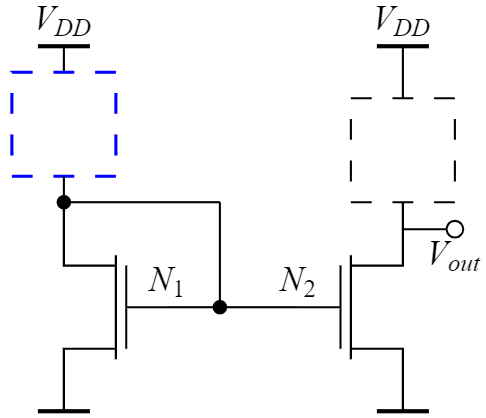
\includegraphics[width=3.5cm]{Stromspiegel_ohneStromquelle_GS.png}\\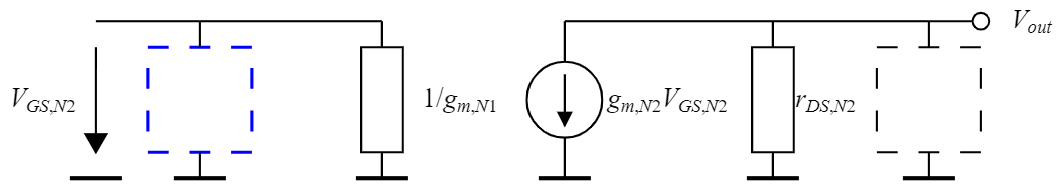
\includegraphics[width=8.5cm]{Stromspiegel_ohneStromquelle_KS.png}
\end{minipage}
\newpage
\section{Einstufiger MOS-Verstärker}
\begin{tabular}{|l|l|l|}
    \hline
    \multicolumn{2}{|l|}{\makecell[l]{\textbf{Verstärker mit Widerstandslast Kleinsignal Ersatzschaltung}}} & \textbf{Verstärker mit MOS-DiodenLast} \\
    \multicolumn{2}{|l|}{\includegraphics[width=0.15\linewidth]{Verstärker mit Widerstandslast.png}\hspace{10pt} \includegraphics[width=0.3\linewidth]{KS_Verstärker mit Widerstandslast.png}} & \includegraphics[width=4.5cm]{Verstärker mit MOS_Diode.png} \\
    \hline
    \makecell[l]{\textbf{Verstärker mit}\\ \textbf{Stromquellenlast Realisierung}} & \makecell[l]{\textbf{Verstärker mit parallelem} \\ \textbf{Eingang (Push-Pull)}} & \textbf{Verstärker mit Stromumlenkung}\\
    \includegraphics[width=0.15\linewidth]{Verstärker mit Stromquellenlast.png} & \includegraphics[width=3.5cm]{Push_Pull Verstärker.png} & \includegraphics[width=4cm]{Verstärker mit Stromumlenkung.png} \\
    \hline
    \textbf{Kaskode mit Widerstandslast} & \textbf{Kaskode mit Stromquellenlast} & \textbf{Gefaltete Kaskode} \\
    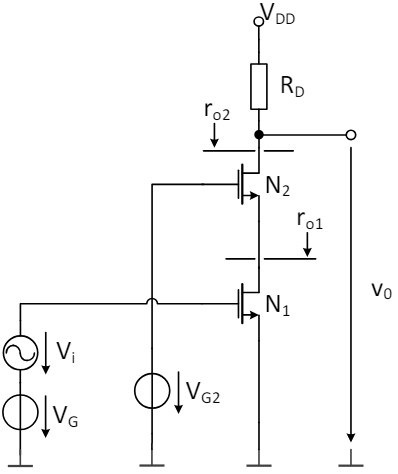
\includegraphics[width=3.5cm]{Kaskode mit Widerstandslast.png} & 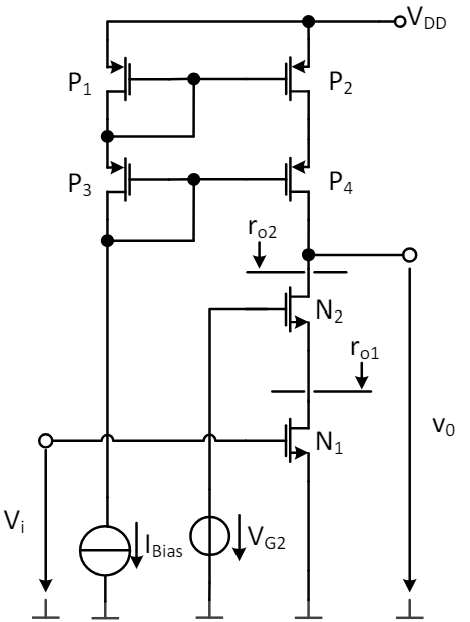
\includegraphics[width=0.15\linewidth]{Kaskode mit Strompiegel Last.png} & 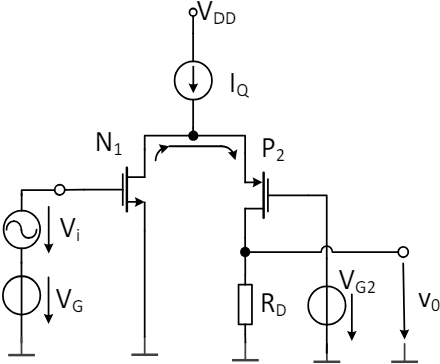
\includegraphics[width=5cm]{Gefaltete Kaskode.png} \\
    \hline
\end{tabular}\\
\begin{tabular}{|l|l|l|l|}
    \hline
    \textbf{Verstärkung mit}  & \textbf{Verstärkung}  & \textbf{Vorteil} & \textbf{Nachteil} \\
    \hline 
    Widerstandslast & \makecell[l]{$a = -\frac{g_m}{\frac{1}{R_D}+g_o}$\\$r_{out} = r_{iD} = \frac{1}{g_o}(1+g_m R_S)+R_S$} & & \\
    \hline
    MOS-Dioden Last & $a = -\frac{\frac{1}{g_{m2}}}{R_S+\frac{1}{g_{m1}}}$\textcolor{brown}{$=-\frac{g_{m1}}{g_{m2}}= \sqrt{\frac{\beta_1}{\beta_2}}$(wenn $R_S = 0$)}& & Nichtlinear \\
    \hline
    Stromquellenlast & $a = -\frac{R_D}{R_S+\frac{1}{g_m}+(R_D+R_S)\frac{g_o}{g_m}}$\textcolor{brown}{$=-\frac{g_{m1}}{\frac{1}{r_Q}+g_{01}}$} & & Frequenzverh. \\
    \hline
    \makecell[l]{parallelem Eingang\\(Push-Pull-Stufe)} & $a= -\frac{g_{m\_N1}+g_{m\_P1}}{g_{0\_N1}+g_{0\_P1}}=-(g_{m\_N1}+g_{m\_P1})\cdot(r_{DS_N1}||r_{DS_P1})$ & Grosse Ströme & Frequenzverh. \\
    \hline
    Stromumlenkung & $a\approx a_i\frac{R_L||r_{DS3}}{R_S+r_{s1}}$ & \makecell[l]{Frequenzverh. \\PSR \\Aussteuerber.} & \makecell[l]{Zusätzlicher \\Strom} \\
    \hline
    Widerstandlast & $a\approx-g_{m1}R_D$ & \makecell[l]{$r_{out}$ sehr hoch \\Frequnzverh.} & Aussteuerber.\\
    \hline
    Gefalteter Kaskode & $a\approx -\frac{g_{m1}}{g_{03}}$& \makecell[l]{PSR \\Aussteuerber.} & \makecell[l]{Zwei Strompfade \\Mehr HW}\\
    \hline
\end{tabular}
\section{Frequenzverhalten von MOS-Verstärker}
\begin{minipage}{0.5\linewidth}
\subsection{Analyse mittels Open-Circuit\\ Time Constant}
\textbf{Bandbreite Bestimmung des verantwortlichen Pols:}
\begin{enumerate}[noitemsep,topsep=0pt]
    \item Setze alle unabhängigen Quellen = 0 (V $\rightarrow$ Kurzschluss, I $\rightarrow$ Leerlauf)
    \item Berechne für alle Kapazitäten die zugehörige Zeitkonstante, wenn alle anderen C = 0.
    \item Bestimme die Bandbreite als Summe der Zeitkonstanten: $\omega_{-3dB} \approx \frac{1}{\sum\tau_k}=\frac{1}{\sum R_kC_k}$
\end{enumerate}
Frequnzen des dominierenden Pols $f_d$ und somit die Bandbreite: $f_d = \frac{1}{2\pi\cdot R_d\cdot C_d}$
\subsection{Kapazitäten}
\textbf{Knotenkapazität hoch (einige pF)}:\\
Knoten mit C als passive Schaltungskomponente\\
\textbf{Knotenkapazität mittel (wenige pF)}:\\
Parasitäre Kapazitäte verstärkt durch Miller-Effekt. Häufig $C_{GD}$ eines verstärkenden Transistors.\\
\textbf{Knotenkapazität tief (fF)}:\\
Knoten mit parasitären Kapazitäten. Von diesen Knoten ist in der Regel der Gate-Knoten mit der höchsten Kapazität belastet.\\
\end{minipage}\hspace{5pt}%
\begin{minipage}{0.5\linewidth}
\textbf{Vorgehen der Frequenzanalyse:}
\begin{enumerate}[noitemsep,topsep=0pt]
    \item DC Verstärkung berechnen (aus Kleinsignalersatzschaltung für tiefe Frequenzen)
    \item Die für die Übertragungsfunktion relevante Pole (und Nullstellen) des Systems finden. Frage: An welchem Knoten befinden sich gleichzeitig ein hoher Widerstand und eine grosse Kapazität, also ein grosses RC-Produkt.
    \item Einzeichnen der einzelnen Pole ( und allenfalls Nullstellen) ins Bode-Diagramm.
\end{enumerate}
Für eine grobe Analyse des Frequenzverhaltens genügt es somit, die Knoten zu suchen, bei denen das grösste RC-Produkt auftritt. Dort wird der dominierende Pol entstehen, welcher einen Abfall des Frequnzganges um 20dB/Dek einleitet.
\subsection{Widerstände}
\textbf{Knotenimpedanz praktisch unendlich (G$\Omega$)}:\\ $r_{iG}\rightarrow \infty$ Gate\\
\textbf{Knotenimpedanz sehr hoch (M$\Omega$)}:\\ $r_{\rm DS} = \frac{1}{g_o}$ Drain wenn Stromquelle\\
\textbf{Kontenimpedanz tief (k$\Omega$)}:\\ $\frac{1}{g_m}$ Drain wenn Diodenschaltung, Source wenn Stromquellenschaltung
\end{minipage}
\begin{minipage}{0.5\linewidth}
\subsection{Miller-Kapazität}
Die Miller-Kapazität $C_m$, die zwischen Ein- und Ausgang eines Verstärkers mit Verstärkung A liegt, erscheint:
\begin{itemize}[noitemsep,topsep=0pt]
    \item multiplizieren mit (1-A) parallel zum Eingang ($C_{mi}$)
    \item multiplizieren mit (1-1/A) parallel zum Ausgang ($C_{mo}$)
\end{itemize}
$C_m$ wird entfernt und durch $C_{mi}$ und $C_{mo}$ ersetzt.\\
Miller-C schiebt $f_d$ nach unten, $f_{nd}$ nach oben.\vspace{5pt}\\
\textbf{Eingangskapazität:}\\
$C_{in} = C_{GS}+A\cdot C_{GD}$
\end{minipage}\hspace{5pt}%
\begin{minipage}{0.5\linewidth}
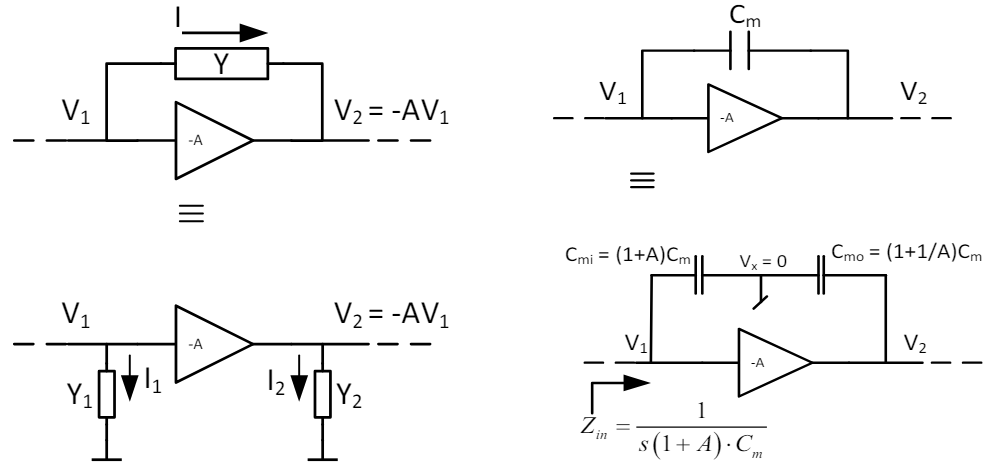
\includegraphics[width=0.9\linewidth]{Miller Approximation.png}
\end{minipage}
\subsection{Typ. Kapazitäten}
\begin{tabular}{|l|l|l|l|l|}
\hline
Arbeitsbereich & $C_{GS}$  & $C_{GD}$  & $C_{SB}$  & $C_{DB}$\\
\hline
\makecell[l]{Gesättigt\\ Typ. Wert} & \makecell[l]{$C_{GS0}+ 2/3C_{oxt}$\\ 33 fF} & \makecell[l]{$C_{GD0}$\\ 1.2fF fF} & \makecell[l]{$C_{jSBt}+ 2/3C_{BCt}$\\ 10 fF} & \makecell[l]{$C_{jDBt}$\\ 7 fF}\\
\hline
\makecell[l]{Ungesättigt\\ Typ. Wert} & \makecell[l]{$C_{GS0}+ 1/2C_{oxt}$\\ 26 fF} & \makecell[l]{$C_{GD0}+ 1/2C_{oxt}$\\ 26 fF} & \makecell[l]{$C_{jSBt}+ 1/2C_{BCt}$\\ 10 fF} & \makecell[l]{$C_{jDBt}+ 1/2C_{BCt}$\\ 10 fF}\\
\hline
\end{tabular}\\
$C_{oxt} = C_{\rm ox}\cdot W \cdot L_{eff}$\hspace{20pt} $C_{BCt} = C_{jBC}\cdot W \cdot L_{eff}$\hspace{20pt} $C_{jSBt} = C_{jSB}\cdot A_S +C_{jswSB}\cdot P_S$ \hspace{20pt} $C_{jDBt} = C_{jDB}\cdot A_D + C_{jswDB} \cdot P_D$\\
Wenn $V_{\rm SB} = 0$, dann $C_{SB}$ ignorieren und $C_{DB} = C_{DS}$
\section{MOS Operationsverstärker}
\begin{minipage}{0.5\linewidth}
\textbf{OTA:} Hohe Eingangsimpedanz, hohe Ausgangsimpedanz.\\
Verhalten einer spannungsgesteuerten Stromquelle.
\end{minipage}%
\begin{minipage}{0.5\linewidth}
\textbf{OpAmp:} Hohe Eingangsimpedanz, tiefe Ausgangsimpedanz.\\
Verhalten einer spannungsgesteuerten Spannungsquelle.
\end{minipage}\vspace{5pt}
\begin{tabular}{l l l l l l}
Aufbau & \makecell[l]{\textbf{Differenzstufe}\\(Eingangsstufe)} & $\rightarrow$ & \makecell[l]{\textbf{Verstärkerstufe}\\(Integrationsstufe)} & $\rightarrow$ & \makecell[l]{\textbf{Leistungsstufe}\\(Ausgangsstufe)}\\
\hline
    & \multicolumn{2}{l}{\makecell[l]{Differenzbildung\\($V^+ - V^-$)\\und Verstärkung}} & \multicolumn{2}{l}{\makecell[l]{Erhöht Verstärkung, meist\\für Bandbreite bestimmt}} & \makecell[l]{Impedanzwandler, leifert\\Strom (fehlt beim OTA)}\\
    \hline
Kaskadierung & \multicolumn{5}{l}{Es können nicht belibig viele Stufen kaskadiert werden. Mind. 90° Phase pro Stufe}
\end{tabular}\vspace{-5pt}\\
\subsection{Differenzstufe}
Eigenschaften der Differenzstufe bei Strong Inversion:\\
\begin{tabular}{l l}
$V_d = \pm\frac{1}{2}\sqrt{\frac{I_Q}{\mu C_{\rm ox}\frac{W}{L}}}$ & Linearität der Diff-Stufe gut. An der Linearitätsgrenzen fliesst $I_D = 0.74 I_Q$ bzw. $I_D = 0.26 I_Q$\\
$V_d = \pm\sqrt{\frac{I_Q}{\mu C_{\rm ox}\frac{W}{L}}}$ & In einem der Zweige fliesst $I_D = 0.93 I_Q$, im anderen $I_D = 0.07 I_Q$\\
$V_d = \pm\sqrt{2}\sqrt{\frac{I_Q}{\mu C_{\rm ox}\frac{W}{L}}}$ & Der gesamte $I_Q$ fliesst in einem der beiden Zweigen.
\end{tabular}\\
\textbf{Wichtig:} Im Arbeitspunkt fliesst gleich viel Strom im linken so wie im rechten Pfad. $I_B = I_{N1} + I_{N2}$
\subsection{Slew-Rate}
\begin{tabular}{|l|l|l|}
\hline
Definition & $SR = \frac{dv_0}{dt} = \frac{I_{out}}{C_L}$\hspace{5pt}$[V/\mu s]$ & \makecell[l]{Maximal mögliche Ausgangsspannungsänderung pro\\Zeiteinheit.}\\
\hline
Differenzstufe & $SR_r = |SR_f| = \frac{I_Q}{C_L}$ & \multirow{2}{*}{\makecell[l]{\textbf{Vorgehen bei mehrstufigem Verstärker:}\\ 1. SR  jeder Verstärkerstufe einzeln untersuchen \\ 2. Auf Ausgang beziehen (SR$\cdot$A)\\3. Verstärkerstufe mit kleinster SR ist dominant}}\\
\makecell[l]{Mehrstufige\\ Verstärker\vspace{5pt}} & $|SR| = \frac{dv_{CL}}{dt}\cdot A = \frac{I_Q}{C_L}\cdot A$ &   \\
\hline
Praxis & \multicolumn{2}{l|}{Designregel für grosse SR: $I_Q$ gross, $C_L$ klein}\\
\hline
\end{tabular}
\subsection{Wichtige Formeln}
\renewcommand{\arraystretch}{2}
\begin{tabular}{|l|l|}
\hline
Transkonduktanz Differenzstufe & \makecell[l]{Ohne Stromspiegel\hspace{10pt}$g_{md} = \frac{\delta i_{out}}{\delta V_d} = \frac{i_{out}}{v_d}=-\frac{g_m}{2}$\\Mit Stromspiegel\hspace{10pt}$g_{md} = \frac{\delta i_{out}}{\delta V_d} = \frac{i_{out}}{v_d}=-g_m$}\\
\hline
Verstärker Differenzstufe & \makecell[l]{Bei Widerstandslast\hspace{10pt} $i_{out}=-\frac{g_m v_d}{2}$\hspace{20pt}$a\approx - \frac{g_m r_{out}}{2}$\\Bei Stromspiegellast\hspace{10pt} $i_{out}=-g_m v_d$\hspace{20pt}$a\approx\ -g_m r_{out}$}\\
\hline
Grenzwert bei Strong Inversion & $a = V_A\sqrt{\frac{\mu C_{\rm ox}\frac{W}{L}}{I_Q}}$ (Bedingung: $a_{EN} = a_{EP}$)\\
\hline
Grenzwert bei Weak Inversion & $a = \frac{V_A}{2 n_M V_{temp}}$\\
\hline
Gain-Bandwith-Product & $GBP = |a|\cdot f_{P1} = -\frac{g_m}{2\pi C_L}$\\
\hline
\makecell[l]{Input Common Mode Range\\($I_{SS}= I_{bias}\frac{(W/L)_{N1}}{(W/L)_{N5}}$)}& \makecell[l]{$V_{inp,max} = (V_{\rm DD}-V_{SS})-V_{GS,P1}-V_{DS,sat,N1}+V_{GS,N1}$\\$V_{inp,min} = V_{SS}+V_{DS,sat,N5}+V_{GS,N1}$ \vspace{5pt}\\Wenn $V_{DS,sat}\approx\sqrt{\frac{2I_D}{\mu C_{\rm ox}\frac{W}{L}}}$ dann gilt:\\$V_{inp,max} = (V_{\rm DD}-V_{SS})-V_{T,P1}-\sqrt{\frac{I_{SS}}{\mu C_{ox,P1}\frac{W}{L}}}+V_{T,N1}$\\$V_{inp,min} = V_{SS}+\sqrt{\frac{2I_{SS}}{\mu C_{ox,N5}\frac{W}{L}}}+V_{T,N1}+\sqrt{\frac{I_{SS}}{\mu C_{ox,N1}\frac{W}{L}}}$}\\
\hline
Common mode rejection ratio & \makecell[l]{$v_{DM} = v_{in1}-v_{in2}$\hspace{20pt}differential mode\\$v_{CM} = \frac{v_{in1}+v_{in2}}{2}$\hspace{20pt} common mode\\$a_{DM}=\frac{v_O}{V_{DM}}\Bigr|_{V_{CM}=0}$\hspace{20pt}(ideal $a_{DM}=\infty$)Gegentaktverstärkung\\$a_{CM}=\frac{v_O}{V_{CM}}\Bigr|_{V_{DM}=0}$\hspace{20pt}(ideal $a_{CM}=0$)Gleichtaktverstärkung\\$CMRR=|\frac{a_{DM}}{a_{CM}}| = \frac{r_q}{r_s}=\frac{g_m}{g_{0b}}$\hspace{20pt}(ideal $CMRR=\infty$)\\mit $r_q$: Innenwiderstand von $I_q$, Gleichtaktunterdrückung}\\
\hline
Power supply rejection ratio & \makecell[l]{$a_{ps}=\frac{\delta v_O}{\delta V_{\rm DD}}|_{V_I=const}=\frac{v_O}{V_{\rm DD}}|_{v_I=0}$\hspace{20pt}(ideal $a_{ps}=0$)\\$PSRR_+=|\frac{a_{DM}}{a_{PS+}}|$\\$PSRR_-=|\frac{a_{DM}}{a_{PS-}}|$}\\
\hline
Offset-Designregeln & \makecell[l]{\textbf{Random Offset}\\Matching von Parametern der Transistoren: Layout für gutes Matching $\rightarrow$\\ Common Centroid, höheres $V_{\rm GS}-V_T$ für Stromspiegel, grosses W/L für\\ Eingangstransistoren.\\\textbf{Systematic Offset}\\Symmetrie der Differenzstufe, gleiche $V_{\rm DS}$ und L der zu einem Stromspiegel\\gehörenden Transistoren, gleiche Stromdichten $\frac{I_D}{W/L}$ in \\Stromspiegeltransistoren. Dies ist auch zwischen der ersten und der zweiten\\Verstärkerstufe zu beachten. (P2, P3) $\frac{I_{D,P3}}{(W/L)_{P3}} = \frac{I_{D,P2}}{(W/L)_{P2}}$}\\
\hline
\end{tabular}
\renewcommand{\arraystretch}{1}
\section{Stabilität von MOS OpAmp}
\begin{minipage}{0.78\linewidth}
Loop-Gain $T(s): T(s)=A(s)\cdot F(s)$\\
\begin{tabular}{|l|l|}
\hline
\makecell[l]{\textbf{Phasenmarge} bei\\$f_{krit} (a_L=1)$} & \makecell[l]{\textbf{Verhalten des Verstärkers}\\(System mit zwei weit auseinanderliegenden Polen)}\\
\hline
$\varphi_M\leq 0^\circ$ & Gegenkoppelter Verstärker schwingt selbständig\\
\hline
$\varphi_M >0^\circ$ & Gedämpftes Überschwingen der Sprungantwort\\
\hline
$\varphi_M =65^\circ$ & Peaking verschwindet. Einziger Überschwinger mit 4.7\% Sprunghöhe\\
\hline
$\varphi_M\geq 75^\circ$ & Kein Überschwingen\\
\hline
\end{tabular}\vspace{5pt}\\
\begin{tabular}{|l|l|}
\hline
\makecell[l]{Regelkreis\\Bodediagramm} & Rückgekoppelter Verstärker\\
\hline
Stabilitätskriterien & \makecell[l]{$\varphi = 180^\circ\Longrightarrow |A(s)\cdot F(s)|<1$\\$|A(s)\cdot F(s)| = 1 \Longrightarrow 180^\circ - \varphi >0; \varphi_M>0^\circ$}\\
\hline
Phasenmarge & $\varphi_M = 180^\circ-\varphi = 90^\circ-\arctan(\frac{GBP}{f_{P2}})$\\
\hline
Designregel & \makecell[l]{Der 1. Pol muss in der ersten Stufe realisiert werdem.\\Der 2. Pol $f_{nd}$ soll bei ca. $3\cdot GBP$ gewählt werden.\\Dies ergibt eine Phasenmarge von 72° und somit\\ kaum Überschwingen}\\
\hline
\end{tabular}
\end{minipage}%
\begin{minipage}{0.2\linewidth}
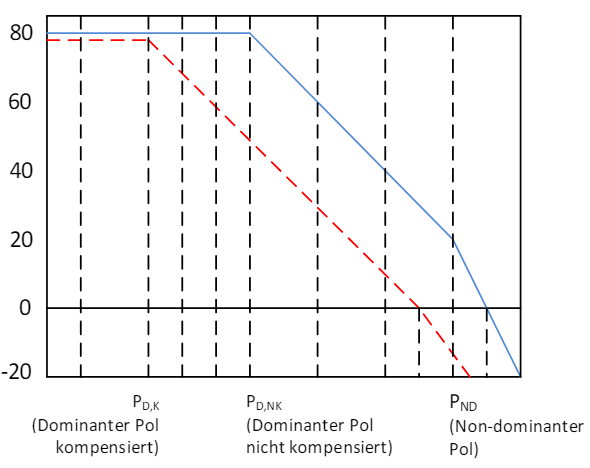
\includegraphics[width=5cm]{Amplitudengang.png} \\ 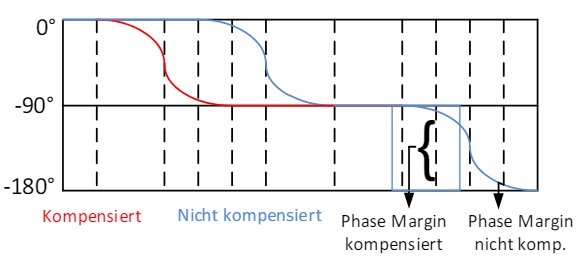
\includegraphics[width=5cm]{Phasenreserve.png}
\end{minipage}
\section{Realisierungsformen von OpAmps}
Ein einstufiger OTA wird bereits durch eine Differenzstufe realisiert. In der Praxis wird ein OTA aber nie so realisiert, da eine Last am Ausgang die Symmetrie der Differenzstufe stört. Der einfachste zweistufige OTA besteht aus einem Differenzverstärker und einem einstufigen Verstärker in Source. Ein Merkmal ist, das der Bias Strom an zwei Stellen gespiegelt wird.\\
\begin{tabular}{l l l}
\textbf{Symmetrischer OTA} & \textbf{Telscopie cascode OTA} & \textbf{Folded cascode OTA}\\
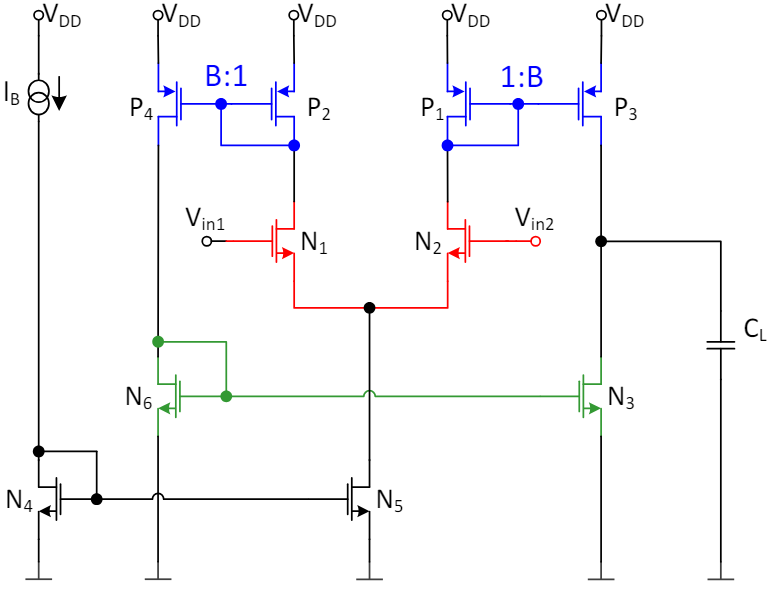
\includegraphics[width=5cm]{Symetrischer OTA.png} & 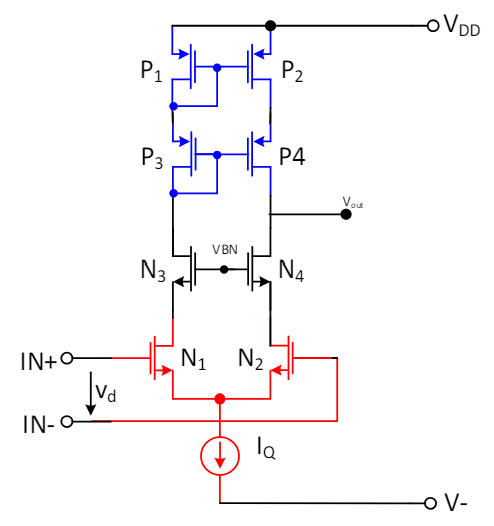
\includegraphics[width=4cm]{Telescopic cascode OTA.png} & 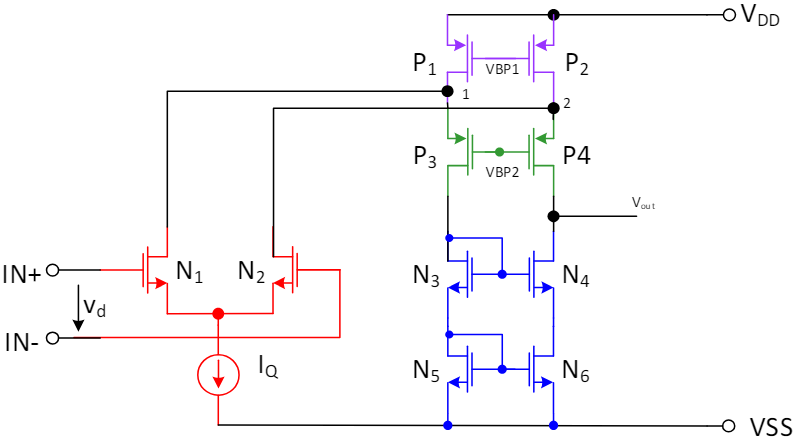
\includegraphics[width=6cm]{Folded cascode OTA.png} \\
\end{tabular}\vspace{10pt}\\
\renewcommand{\arraystretch}{1.8}
\begin{tabular}{|l|l|l|l|l|l|}
\hline
OTA-Typ & $a$ & $r_{out}$ & $BW$ & $GBP$ & Bemerkung \\
\hline
Symmetrischer OTA & $B\cdot g_{m,N1}\cdot r_{out}$ & $(r_{DS,N3}||r_{DS,P3})$ & $\frac{1}{2\pi\cdot r_{out}C_L}$ & $B\cdot \frac{g_{m,N1}}{2\pi\cdot C_L}$ & \\
\hline
Telescopie Cascode & $-g_{m,N1,2}\cdot r_{out}$ & $(r_{K,N}||r_{K,P})$ & $\frac{1}{2\pi \cdot r_{out}C_L}$ & $\frac{g_{m,N1,2}}{2\pi \cdot C_L}$ & \makecell[l]{$r_{K,N,K,P}\approx r_{\rm DS}\cdot (2+g_m\cdot r_{\rm DS})$\\Vorteil: Hohe Verstärkung,\\ Geringer Stromverbrauch}\\
\hline
Folded Cascode & $g_{m,N1,2}\cdot r_{out}$ & $(r_{K,N}||r_{K,P})$ & $\frac{1}{2\pi\cdot r_{out}C_L}$ & $\frac{g_{m,N1,2}}{2\pi\cdot C_L}$ & \makecell[l]{Vorteil: Hohe Verstärkung\\Nachteil: Hoher Stromverbrauch}\\
\hline
\end{tabular}\vspace{10pt}\\
\textbf{Miller OTA -Desinggleichungen}\\
\renewcommand{\arraystretch}{1.5}
\begin{tabular}{|l|l|l|}
\hline
Schaltung: & \multicolumn{2}{l|}{Wichtige Parameter: (Mit $C_c$ von Knoten 2 nach Knoten 3)} \\
\hline
\multirow{7}{*}{\includegraphics[width=6cm]{Miller OTA.png}} & Dominanter Pol: & $f_{d} = f_{K2} = \frac{1}{2\pi R_{K2}(C_{N2}+a_2C_c)} \approx \frac{1}{2\pi R_{K2}\cdot a_2C_c}$\\
\cline{2-3}
                  & Nondominanter Pol: & $f_{nd} = f_{K3} = \frac{1}{2\pi R_{K3}C_L}\approx\frac{g_{m,P3}}{2\pi C_L}$\\
\cline{2-3}
                  & 3dB Bandbreite: & $BW\approx f_d = f_{K2} = \frac{1}{2\pi R_{K2}\cdot a_2C_c}$\\
\cline{2-3}
                  & Phasenmarge: & $\varphi_M = 90^\circ-\arctan(\frac{GBP}{f_{nd}})$\\
\cline{2-3}
                  & \makecell[l]{Gain-Bandwitdh\\ Produkt:} & $GBP = a_1\cdot a_2\cdot f_d = \frac{g_{m,N1,2}\cdot R_{K2}\cdot g_{m,P3}\cdot R_{K3}}{2\pi R_{K2}\cdot a_2C_c} = \frac{g_{m,N1}}{2\pi C_c}$\\
\cline{2-3}
                  & zusätzliche Nullstelle: & $f_z \approx \frac{g_{m,P3}}{2\pi C_c}$\\
\cline{2-3}
                  & Verstärkung: & \makecell[l]{$a = a_1\cdot a_2 = g_{m,N1,2}\cdot R_{K2}\cdot g_{m,P3}\cdot R_{K3} = $\\$g_{m,N1,2}(r_{DS,N2}||r_{DS,P2})\cdot g_{m,P3}(r_{DS,N3}||r_{DS,N3}||R_L)$}\\
\cline{2-3}
                  & \multicolumn{2}{l|}{Wichtige Parameter: (Mit $C_1$ von Knoten 2 nach GND)}\\
\cline{2-3}
                 & Dominanter Pol: & $f_{d} = \frac{1}{2\pi R_{K2}\cdot C_1}$\\
\hline
\end{tabular}
\newpage
\section{Spannungsreferenzen}
In vielen Anwendungen benötigt man eine Spannung, die unabhängig von Betriebsspannungsschwankungen oder Temperaturänderungen ist. Eine solche Spannungsquelle wird als Spannungsreferenz bezeichnet.\\
\begin{tabular}{l l l}
\textbf{Spannungsteiler} & \textbf{MOS-Diode} & \textbf{Bandgap-Spannungsreferenz} \\
\includegraphics[width=2.5cm]{Spannungsteiler.png} &
\includegraphics[width=3cm]{MOS-Spannungsreferenz.png} &
\includegraphics[width=4cm]{Bandgap Schaltung.png}\\
\end{tabular}\\
\begin{tabular}{|l|l|l|l|}
\hline
S = Sensitivität & \textbf{Temperatur} & \textbf{VDD/VSS} & \textbf{Prozessvariation}\\
\hline
Spannungsteiler & S klein & S = 1 & S = klein\\
\hline
MOS-Diode & S klein & S < 1 & S: Darf nicht vernachlässigt werden\\
\hline
Bandgap & \makecell[l]{Abhängig von R\\ und von $V_{temp} = \frac{kT}{e}$} & 0 (unabhängig von VDD/VSS) & klein\\
\hline
\end{tabular}
\subsection{Bandgap-Spannungsreferenzen}
In vielen Anwendungen benötigt man eine Spannung, die unabhängig von Betriebsspannungsschwankungen oder Temperaturänderungen ist. Die Bandgap ist eine Möglichkeit, eine Spannungsreferenz zu erhalten.\\
\begin{minipage}{0.5\linewidth}
\includegraphics[width=8cm]{Bandgap Spannungsreferenz.png}
\end{minipage}%
\begin{minipage}{0.5\linewidth}
\boxed{V_{ref} = V_D + K\cdot V_{temp}}\\
\end{minipage}
\subsection{Realisierung}
\begin{minipage}{0.3\linewidth}
\includegraphics[width=4cm]{Bandgap Schaltung.png}
\end{minipage}%
\begin{minipage}{0.7\linewidth}
\boxed{V_{ref} = V_D + K\cdot V_{temp}}\\
\boxed{V_{EB} = V_{temp}\ln\Bigl(\frac{-I_C}{I_s'A_E}\Bigr) \text{mit $I_s'$ = Sättigungsstrom pro Flächeneinheit}}\\
\boxed{K = \frac{R_2}{R_3}\cdot \ln\Bigl(\frac{R_2}{R_1}\frac{A_2}{A-1}\Bigl)}   
\end{minipage}
\subsection{Offsetfehler}
Die Bandgap-Schaltung hat den Nachteil, dass $V_{ref}$ stark vom Offset-Spannungsfehler $V_{os}$ des Opamp abhängt.\\
\boxed{V_{ref} = V_{EV1} + \frac{R_2}{R_3}\cdot V_{temp}\cdot\Bigl[\frac{R_2 A_2}{R_1 A_1}\cdot\Bigl(1-\frac{V_{eff}}{R_2 I_2}\Bigr)\Bigr]-\Bigl(1+\frac{R_2}{R_3}\Bigr)\cdot V_{os}}
\subsection{Diverses}
\textbf{dB Umrechner}\\
\boxed{x = 10\cdot\log(P)}\hspace{5pt} Leistungsintensität\\
\boxed{x = 20\cdot\log(A)}\hspace{5pt} Amplitudenintensität\\